\documentclass[a4paper,12pt]{memoir}
%%%%%%%%%%%%%%%%%%%%%%%%%%%%%%%%%%%%%%%%%%%%%%%%%%%%%%%%%%%%%%%%%%%%%%%%%%%%%
% EDIT HERE!!!
%%%%%%%%%%%%%%%%%%%%%%%%%%%%%%%%%%%%%%%%%%%%%%%%%%%%%%%%%%%%%%%%%%%%%%%%%%%%%
\def\candidate{First Last} % Your name
\def\thesistitle{A Very Very Long Title of the Super-Wonderful PhD Thesis Should Be Avoided If Possible} % Be as short as you can!! No more than 10 words
\def\keywords{Subject 1, Subject 2}
\def\advisor{Prof. First Last} 
\def\headphdprogram{Prof. First Last}
\def\refereeone{\textnormal{Prof. First Last}, \textit{institution}}
\def\refereetwo{\textnormal{Prof. First Last}, \textit{institution}}
\def\ciclo{XXXII}
% End EDIT
%%%%%%%%%%%%%%%%%%%%%%%%%%%%%%%%%%%%%%%%%%%%%%%%%%%%%%%%%%%%%%%%%%%%%%%%%%%%%

\usepackage[utf8]{inputenc}

\addtolength{\textwidth}{40pt}
\addtolength{\foremargin}{-40pt}
\addtolength{\spinemargin}{-40pt}
\setlrmarginsandblock{2.8cm}{2.8cm}{*}
\setulmarginsandblock{2.8cm}{*}{1}
\checkandfixthelayout%
\headsep=30pt
\linespread{1.1}

\usepackage[draft,inline,nomargin]{fixme}
\usepackage[round]{natbib}
\usepackage{graphicx}
\graphicspath{{./Figures/}}
\usepackage{xcolor}
\usepackage[pdftex]{hyperref}
\hypersetup{
  hidelinks,
  linkbordercolor=white,
  citebordercolor=white,
  urlbordercolor=white,
  filebordercolor=white}

\let\footruleskip\undefined %correct bug in footruleskip definition in
                            %memoir and fancyhdr
\usepackage{fancyhdr}
\pagestyle{fancy}
\renewcommand{\chaptermark}[1]{\markboth{#1}{}}
\renewcommand{\sectionmark}[1]{\markright{\thesection\ #1}}
\fancyhf{}
\fancyhead[LE,RO]{\fontfamily{phv}\selectfont\thepage}
\fancyhead[LO]{\rightmark}
\fancyhead[RE]{\fontfamily{phv}\selectfont\bfseries\leftmark}
\renewcommand{\headrulewidth}{0.1pt}
\renewcommand{\footrulewidth}{0pt}

\usepackage{verbatim}
\usepackage{url}
\usepackage{hyphenat}

\usepackage{amsmath,amsfonts,amssymb,amsthm}
\usepackage{latexsym}
\usepackage{array}
\usepackage{tocbibind}
\usepackage{listings}
\usepackage[retainorgcmds]{IEEEtrantools}

\usepackage{algorithmic}
\usepackage{algorithm2e}
\usepackage{color}
\usepackage{textcomp}
\usepackage{stackengine}

\hypersetup{ 
  pdfpagelayout=SinglePage, % default
  pdfpagemode=UseOutlines, % default
  bookmarksopen, % default
  bookmarksopenlevel=2, % default;
  pdftitle={\candidate's PhD thesis},
  pdfauthor={\candidate},
  pdfsubject={\thesistitle},
  pdfkeywords={PhD Program in Smart Computing, \keywords}
}

\usepackage[english]{babel}
\usepackage{blindtext}

\usepackage[sc]{mathpazo} % for maths
\usepackage{tgpagella} % as main font
\usepackage{nimbussans} % Helvetica

%\usepackage{makeidx}
%\makeindex

\usepackage{multirow}
\usepackage{acronym}
\usepackage{amsmath}
\usepackage{amssymb}
\usepackage{mathtools}
\usepackage{bm}
% \usepackage{subfigure}
\usepackage{subfig}
\usepackage{cleveref}
\usepackage{tikz}
\usetikzlibrary{positioning}
\usetikzlibrary{calc}


\definecolor{UFblue}{RGB}{12, 71, 123}



\newcommand{\svm}{\textbf{\emph{U-SVM}}}
\newcommand{\svmb}{\textbf{\emph{B-SVM}}}
\newcommand{\lstmng}{\textbf{\emph{B-LSTM}}}
\newcommand{\lstmc}{\textbf{\emph{G-CRNN}}}
\newcommand{\lstmb}{\textbf{\emph{G-LSTM}}}
\newcommand{\maxp}{\textbf{\emph{G-MAX}}}
\newcommand{\softmax}{\textbf{\emph{G-ATT}}}
\newcommand{\maxi}{\textbf{\emph{G-MAXi}}}
\newcommand{\softmaxi}{\textbf{\emph{G-ATTi}}}
\newcommand{\maxh}{\textbf{\emph{G-MAXh}}}
\newcommand{\softmaxh}{\textbf{\emph{G-ATTh}}}
\newcommand{\bert}{\textbf{\emph{BERT}}}
\newcommand{\gru}{\textbf{\emph{G-GRU}}}
\newcommand{\xgb}{\textbf{\emph{B-XGB}}}


\newcommand{\site}{Main-site}
\newcommand{\fullSite}{Full-site}
\newcommand{\type}{Type}
\newcommand{\behaviour}{Behavior}

\newcommand{\matr}[1]{\bm{#1}}
\newcommand{\vect}[1]{\bm{#1}}
\newcommand{\dist}[1]{\mathcal{#1}}

\newtheorem{definition}{Definition}[section]
\newtheorem{lemma}[definition]{Lemma}
\newtheorem{corollary}[definition]{Corollary}
\newtheorem{theorem}[definition]{Theorem}

\def\RSet{\mathbb{R}}
\def\NSet{\mathbb{N}}
\def\XSet{\mathbb{X}}
\def\YSet{\mathbb{Y}}
\def\HSet{\mathbb{H}}
\def\prob{\mathbb{P}}
\def\expect{\mathbb{E}}
\def\define{\overset{\underset{\mathrm{def}}{}}{=}}

\DeclareMathOperator*{\argmax}{arg\,max}
\DeclareMathOperator*{\argmin}{arg\,min}

\def\loss{\mathcal{L}}

\acrodef{han}[HAN]{Hierarchical Attention Network}
\acrodef{max}[MM]{Max Model}
\acrodef{softmax}[AM]{Attention Model}
\acrodef{maxi}[MMi]{Max Model interpretable}
\acrodef{maxh}[MMh]{Max Model hierarchical}
\acrodef{softmaxh}[AMh]{Attention Model hierarchical}
\acrodef{srm}[SRM]{Structural Risk Minimization}
\acrodef{vcd}[VC-dimension]{Vapnik-Chervonenkis dimension}
\acrodef{pac}[PAC]{Probably Approximately Correct}
\acrodef{iid}[i.i.d.]{indipendently and identically distributed}
\acrodef{ml}[ML]{Machine Learning}
\acrodef{ai}[AI]{Artificial Intelligence}
\acrodef{erm}[ERM]{Empirical Risk Minimization}
\acrodef{rtt}[RTT]{Registro Tumori della Toscana, Tumor Registry of Tuscany}
\acrodef{icdo}[ICD-O]{International Classification of Diseases for Oncology}
\acrodef{icdo1}[ICD-O-1]{International Classification of Diseases for Oncology, first edition}
\acrodef{icdo3}[ICD-O-3]{International Classification of Diseases for Oncology, third edition}
\acrodef{hdr}[HDR]{Hospital Discharge Register}
\acrodef{ehr}[EHR]{Electronic Health Record}
\acrodef{cdf}[CDF]{Cumulative Distribution Function}
\acrodef{an}[AN]{Artificial Neuron}
\acrodef{ann}[ANN]{Artificial Neural Network}
\acrodef{cnn}[CNN]{Convolutional Neural Network}
\acrodef{rnn}[RNN]{Recurrent Neural Network}
\acrodef{mlp}[MLP]{Multilayer Perceptron}
\acrodef{lstm}[LSTM]{Long Short-Term Memory}
\acrodef{sgd}[SGD]{Stochastic Gradient Descend}
\acrodef{glove}[GloVe]{Global Vectors}
\acrodef{nb}[NB]{Naive Bayes}
\acrodef{svm}[SVM]{Support Vector Machine}
\acrodef{tfidf}[TF-IDF]{Term-Frequency Inverse-Document-Frequency}
\acrodef{map}[MAP]{Mean Average Precision}
\acrodef{relu}[ReLU]{Rectified Linear Unit}
\acrodef{gru}[GRU]{Gated Recurrent Unit}
\acrodef{nlp}[NLP]{Natural Language Processing}
\acrodef{bert}[BERT]{Bidirectional Encoder Representations from Transformers}
\acrodef{mlm}[MLM]{Masked Language Model}
\acrodef{nsp}[NSP]{Next Sentence Prediction}

\newcommand\floatwidth{0.9\textwidth}
\newcommand\attTableIcdoWidth{2.5cm}
\newcommand\attTableTextWidth{10cm}
\newlength\lunderset
\newlength\rulethick
\lunderset=1.7pt\relax
\rulethick=.8pt\relax
\def\stackalignment{l}
\newcommand\att[4][1]{\setbox0=\hbox{#2}%
  \stackunder[#1\lunderset-\rulethick]{\strut#2}{\color{#3!#4}\rule{\wd0}{\rulethick}}}

\definecolor{att}{rgb}{0, 1, 0}
\definecolor{attb}{rgb}{1, 0, 0}
\newcommand{\attvisB}[3]{\tikz[overlay]\node[fill=att!#2,inner sep=1pt, anchor=text, rectangle, rounded corners=1mm,draw=attb!#3] {#1};\phantom{#1}}

\makeatletter
  \providecommand*\setfloatlocations[2]{\@namedef{fps@#1}{#2}}
\makeatother
\setfloatlocations{figure}{htbp}
\setfloatlocations{table}{htbp}

\newcommand{\dataLabelScale}{0.6}
\newcommand{\schemeNodeDistance}{0.5cm}

\tikzstyle{every neuron}=[circle, draw, minimum size=1cm]
\tikzstyle{bias}=[circle,draw]
\tikzstyle{operation}=[circle,draw]
\tikzstyle{activation}=[draw]
\tikzstyle{layer}=[draw,minimum size=1cm]
\tikzstyle{delay}=[draw,minimum size=0.5cm,fill=black]
\tikzstyle{neuron missing}=[draw=none, scale=4,text height=0.333cm,execute at begin node=\color{black}$\vdots$]
\tikzstyle{vmissing}=[draw=none, scale=4,text height=0.333cm,execute at begin node=\color{black}$\vdots$]
\tikzstyle{hmissing}=[draw=none, scale=4,text width=0.41cm,execute at
begin node=\color{black}$\cdots$]
\tikzstyle{line}=[]
\tikzstyle{arrow}=[->, >=stealth]
\tikzstyle{arrowInverse}=[<-, >=stealth]
\tikzstyle{vectorLine}=[line width=0.6mm]
\tikzstyle{vectorArrow}=[->, >=stealth, line width=0.6mm]
\tikzstyle{border}=[draw]
\tikzstyle{dataBlock}=[draw,minimum size=1cm, minimum height=2cm, double copy shadow={shadow xshift=-0.5ex, shadow yshift=-0.5ex}, fill=white]
\tikzstyle{layer}=[draw,minimum height=2cm]
\tikzstyle{joined}=[join=by {->}]
\tikzstyle{support}=[coordinate,join=by {-}]
\tikzstyle{dataLabel}=[scale=\dataLabelScale]

\newcommand\nodeInput{} % just for safety
\def\nodeInput(#1){%
  \node[dataBlock,joined,scale=\dataLabelScale] (#1) {$200$};
}

\newcommand\nodeEmbedding{} % just for safety
\def\nodeEmbedding(#1){%
  \node[layer,joined] (#1) {\rotatebox{90}{Embed}};
}

\newcommand\nodeGlove{} % just for safety
\def\nodeGlove(#1){%
  \node[layer,joined] (#1) {\rotatebox{90}{GloVe}};
}

\newcommand\nodeConv{} % just for safety
\def\nodeConv(#1){%
  \node[layer,joined] (#1) {\rotatebox{90}{Conv 2}};
}

\newcommand\nodeLstm{} % just for safety
\def\nodeLstm(#1){%
  \node[layer,joined] (#1) {\rotatebox{90}{Bi. LSTM}};
}

\newcommand\nodeAvg{} % just for safety
\def\nodeAvg(#1){%
  \node[layer,joined] (#1) {\rotatebox{90}{Avg pool}};
}

\newcommand\nodeRelu{} % just for safety
\def\nodeRelu(#1){%
  \node[layer,joined] (#1) {\rotatebox{90}{ReLU}};
}

\newcommand\nodeSoftmax{} % just for safety
\def\nodeSoftmax(#1){%
  \node[layer,joined] (#1) {\rotatebox{90}{Softmax}};
}

%%% Local Variables:
%%% mode: latex
%%% TeX-master: "thesis"
%%% End:


\begin{document}
\hypersetup{pageanchor=false}
\thispagestyle{empty}
\pagenumbering{gobble}

{
  \fontfamily{phv}\selectfont

  \noindent
  \hspace*{-2.5cm}\includegraphics[height=4cm]{firenze}
  \vskip 1.6ex

  \noindent
  \hspace*{1.3cm}{\large \textsc{PhD Program in Smart Computing}}

  \noindent
  \hspace*{1.3cm}{\textsc{Dipartimento di Ingegneria dell'Informazione (DINFO)}}

  \vfill
  \noindent
  \hspace*{1.3cm}
  \parbox{1.0\textwidth}{
    {\fontsize{30}{38}\selectfont \color{UFblue} \textbf{\nohyphens{\thesistitle}}\par}
    \vspace{6cm}
    \begin{flushright}
      \LARGE \textbf{\candidate}\\
      \vspace{8mm}
      \small Dissertation presented in partial fulfillment of the
      requirements\\
      for the degree of Doctor of Philosophy in Smart
      Computing
    \end{flushright}
  }
}

\newpage
\setulmarginsandblock{3.5cm}{3.5cm}{1}
{%
  \fontfamily{phv}
  \noindent
  \textit{PhD Program in Smart Computing}\\
  \textit{University of Florence, University of Pisa, University of Siena}

  \vfill
  \noindent
  % {\HUGE \textbf{\nohyphens{\thesistitle}}}
  {\fontsize{32}{38}\selectfont \textbf{\nohyphens{\thesistitle}}\par}
  \vfill
  \noindent
  {\Large \textbf{\candidate}}
}
\vfill
{
  % These are the required signatures according to unifi regulations
  \noindent
  \begin{minipage}{0.4\linewidth}
    \noindent
    {\fontfamily{phv}\textbf{Advisor:}}\\
    \vspace{7mm}
    \hrule
    \vspace{2mm}
    \advisor
  \end{minipage}

  \vspace{15mm}
  \noindent
  \begin{minipage}{0.4\linewidth}
    \noindent
    {\fontfamily{phv}\textbf{Head of the PhD Program:}}\\
    \vspace{7mm}
    \hrule
    \vspace{2mm}
    \headphdprogram
  \end{minipage}

  \vspace{15mm}

  % No signatures required here
  \noindent
  {\fontfamily{pag}\textbf{Evaluation Committee:}}\\
  \refereeone\\
  \refereetwo
}

\begin{center}
  \rule{\linewidth}{0.5mm}
  \fontfamily{pag}
  \ciclo\ ciclo --- October \number\the\year
  % \noindent Copyright~\copyright~\number\the\year~by \candidate.
\end{center}
\thispagestyle{empty}\null\vfil

\frontmatter
\newpage
\thispagestyle{empty}
%%%%%%%%%%%%%%%%%%%%%%%%%%%%%%%%%%%%%%%%%%%%%%%%%%%%%%%%%%%%%%%%%%%%%%%%%%%%% 
% EDIT HERE!!!
%%%%%%%%%%%%%%%%%%%%%%%%%%%%%%%%%%%%%%%%%%%%%%%%%%%%%%%%%%%%%%%%%%%%%%%%%%%%% 
\begin{flushright}
  \textit{To XXXXX} % Optional dedication
\end{flushright}
\null\vfil
% End EDIT
%%%%%%%%%%%%%%%%%%%%%%%%%%%%%%%%%%%%%%%%%%%%%%%%%%%%%%%%%%%%%%%%%%%%%%%%%%%%%
\newpage
\section*{Acknowledgments}
First of all, I would like to express my gratitude to my advisor
Prof. Paolo Frasconi for his expert guidance, for the important
insights he shared about the field of AI and the always new and
inspiring inputs about research.

Second, I would like to thank Leonardo Ventura, Prof. Gianni Amunni,
and \mbox{ISPRO} for giving me the opportunity to work with their data and
making this work of thesis possibile.

Thanks to Prof. S{\o}ren Brunak and Prof. Beatrice Lazzerini for
helping me advancing my 
research. 

I’m grateful to Prof. Enrico Vicario for introducing me to this
doctorate and to Prof. Simone Marinai for his precious advice.

A special thanks goes to the people who shared the AI-Team lab and the
Ph.D life with me. In alphabetical order: Daniele Baracchi, Samuele
Capobianco, Alessandro Lazzeri, Francesco Orsini, Giulia Pellegrini,
Dasara Shullani,
Alessandro Tibo, La Ode Toresano, Amin Zadenoori, and Zahra Ziran.

I would like to thank all my friends that were always there to support
me, root for me and cheer me up in moments of crisis and
doubt. Special mentions: Andrea Benassai, Vito Bonelli, Giulia
Bondielli, Giulia Bono, Tiberio Uricchio. Thanks to my dear family
Mauro, Rosa, and Simone for their presence and affection throughout my
whole life. Thanks to Fede for all the help that she gave me in this
thesis and in my whole life and for loving me dearly. Last but not
least, thanks to Spallina for accompanying me from the start to the
end of my academic path.


\newpage
\begin{abstract}
  \blindtext % Put your abstract here - don't exceed one page
\end{abstract}
\newpage

\pagenumbering{arabic}
\hypersetup{pageanchor=true}

\mainmatter
\tableofcontents
% \newpage\listoffigures% optional
% \newpage\listoftables% optional

%%%%%%%%%%%%%%%%%%%%%%%%%%%%%%%%%%%%%%%%%%%%%%%%%%%%%%%%%%%%%%%%%%%%%%%%%%%%%
% EDIT HERE!!!
%%%%%%%%%%%%%%%%%%%%%%%%%%%%%%%%%%%%%%%%%%%%%%%%%%%%%%%%%%%%%%%%%%%%%%%%%%%%%
\chapter{Introduction}
\label{ch:introduction}

\section{Machine Learning}

\section{Neural Networks}
In our work we used a specific kind of \ac{rnn}: \ac{lstm}.
\acp{rnn} are a class of \acp{ann} where the connections are not only
sequential from one layer to the subsequent, but instead they form
loops. 

\subsection{\acf{ann}}
\begin{figure}
  \centering
  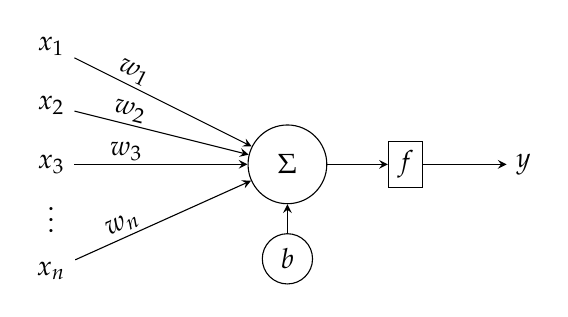
\begin{tikzpicture}[x=1.5cm, y=1.5cm]
    \node [] (input-1) at (0,0.5) {$x_1$};
    \node [] (input-2) at (0,0) {$x_2$};
    \node [] (input-3) at (0,-0.5) {$x_3$};
    \node [] (input-missing) at (0,-0.9) {$\vdots$};
    \node [] (input-n) at (0,-1.4) {$x_n$};

    \node [every neuron] (neuron) at (2,-0.5) {$\Sigma$};
    \node [bias] (bias) at (2,-1.3) {$b$};

    \node [activation] (act) at (3,-0.5) {$f$};
    \node [] (output) at (4,-0.5) {$y$};
    
    \foreach \i in {1,...,3,n}
    \draw [arrow] (input-\i) -- (neuron)
    node [above=-0.05, pos=0.3, sloped] {$w_\i$};

    \draw [arrow] (bias) -- (neuron);

    \draw [arrow] (neuron) -- (act);
    \draw [arrow] (act) -- (output);
  \end{tikzpicture}
  \caption{Artificial neuron.}
  \label{fig:neuron}
\end{figure}
An \ac{ann} is a model that performs elaboration in a way that
mimics the brain functioning. The base unit is the \ac{an}, also called
perceptron, of
\cref{fig:neuron}. It performs the weighted sum of the inputs
$x_1,\dots,x_n$, shifted by a bias $b$, followed by an activation
function $f$. If we add a dummy input $x_0=1$ and rename the bias
$b=w_0$, we can express the computation of the \ac{an} as in
\cref{eq:anComp}:
\begin{equation}\label{eq:anComp}
  y = f(\sum_{i=0}^n w_i x_i).
\end{equation}

The activation function $f$ can be of different types, the most common are:
\begin{itemize}
\item Softmax;
\item ReLU;
\item TanH;
\item Sigmoid;
\item Linear;
\end{itemize}

\begin{figure}
  \centering
  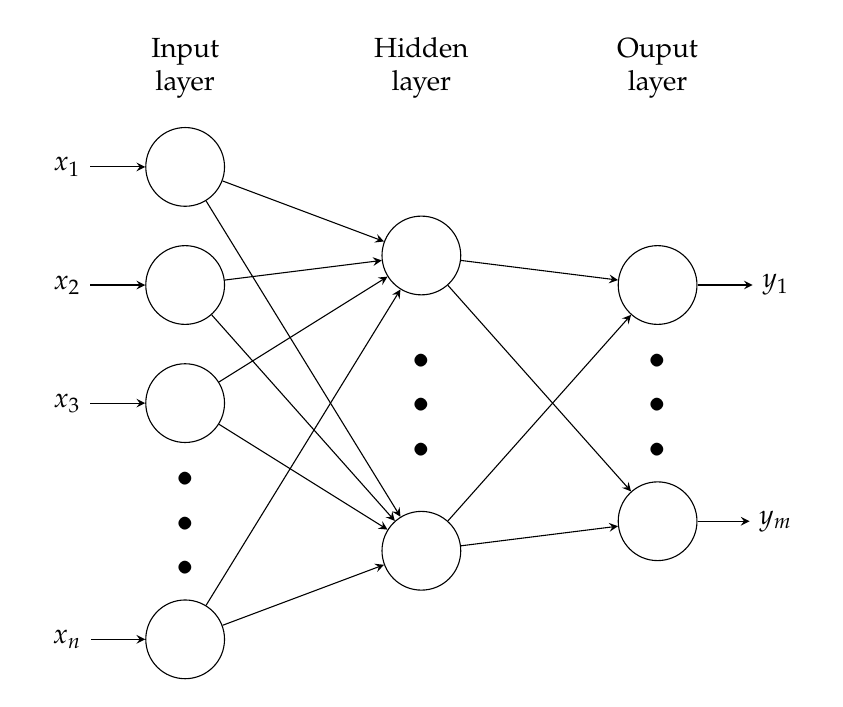
\begin{tikzpicture}[x=1.5cm, y=1.5cm]
    \foreach \m/\l [count=\y] in {1,2,3,missing,4}
    \node [every neuron/.try, neuron \m/.try] (input-\m) at (0,2.5-\y) {};

    \foreach \m [count=\y] in {1,missing,2}
    \node [every neuron/.try, neuron \m/.try ] (hidden-\m) at (2,2-\y*1.25) {};

    \foreach \m [count=\y] in {1,missing,2}
    \node [every neuron/.try, neuron \m/.try ] (output-\m) at (4,1.5-\y) {};

    \foreach \l [count=\i] in {1,2,3,n}
    \node[] (x-\i) at ($(input-\i)-(1,0)$) {$x_\l$};

    \foreach \l [count=\i] in {1,2,3,n}
    \draw [arrow] (x-\i) -- (input-\i);
    %\draw [arrowInverse] (input-\i) -- ++(-1,0)
    %node [above, midway] {$I_\l$};

    %\foreach \l [count=\i] in {1,n}
    %\node [above] at (hidden-\i.north) {$H_\l$};

    \foreach \l [count=\i] in {1,m}
    \node[] (y-\i) at ($(output-\i)+(1,0)$) {$y_\l$};
    
    \foreach \l [count=\i] in {1,n}
    \draw [arrow] (output-\i) -- (y-\i);
    %\draw [arrow] (output-\i) -- ++(1,0)
    %node [above, midway] {$O_\l$};

    \foreach \i in {1,...,4}
    \foreach \j in {1,...,2}
    \draw [arrow] (input-\i) -- (hidden-\j);

    \foreach \i in {1,...,2}
    \foreach \j in {1,...,2}
    \draw [arrow] (hidden-\i) -- (output-\j);

    \foreach \l [count=\x from 0] in {Input, Hidden, Ouput}
    \node [align=center, above] at (\x*2,2) {\l \\ layer};

  \end{tikzpicture}
  \caption{\acf{mlp} with one hidden layer.}
  \label{fig:ann}
\end{figure}
\acp{an} are organized in network structures. The basic layout of
an  \ac{ann} is the \acf{mlp} structured in layers like in
\cref{fig:ann}. Each \ac{an} of each layer is connected to all the
outputs of the previous layer. The first layer is connected to the
inputs of the \ac{ann} and the output of the last layer is also the
output of the network. The execution of the \ac{mlp} is feed forward:
\begin{enumerate}
\item the input values $x_{0,1},\dots x_{0,n}$ are presented to the
  network and it is the input of the first layer;
\item  the computation is 
  carried one layer at a time, where each neuron $i$ of the layer $l$
  calculates the value $y_{l,i}$ of the intermediate output
  $y_{l,1},\dots,y_{l,m}$;
\item the intermediate output $y_{l,1},\dots,y_{l,m}$ of the layer $l$
  becomes the 
  input $x_{l+1,1},\dots,x_{l+1,m}$ of the subsequent layer $l+1$,
  unless $l$ is the last layer - in that case the output of $l$ is the
  output $y_1,\dots,y_m$ of the \ac{mlp}.
\end{enumerate}

The weights of the \acp{an} are initialized to random values and, in order
to have meaningful outputs, the \ac{ann} needs to be trained. In a
supervised learning framework the dataset is composed of the matrices
$\matr{X}$ ($N\times n$) of the $N$ inputs $x_{i,j}$, and $\matr{Y}$
($N\times m$) of 
the corresponding outputs $y_{i,j}$. The
training process is called \emph{backpropagation} and it is organized in a
succession of phases. For each phase $p$ there are two steps:
\begin{description}
\item[execution] where an input $x_{p,1},\dots x_{p,n}$ is given to
  the network and an output $\hat{y}_{p,1},\dots,\hat{y}_{p,m}$ is calculated;
\item[weight update] where is calculated the error between
  $\hat{y}_{p,1},\dots,\hat{y}_{p,m}$ and the correct output
  $y_{p,1},\dots,y_{p,m}$, this error is back propagated through all
  the layers and a correction $\Delta w_i$ is calculated for each weight $w_i$ of
  the network, in
  order to minimize the error surface in the space of the weights.
\end{description}
In detail, to calculate the weights $\vect{w}^{(p+1)}$ for the next
phase $p+1$, it is 
sufficient to determine the gradient of 
the error surface in the current point $\vect{w}^{(t)}$ in order to
apply an optimization method like \ac{sgd}.

\subsection{\acf{rnn}}
\acp{rnn} are specialized versions of \ac{ann} for sequences. They
exhibit an
internal state $\vect{h}$ that changes during the training and that
recursively depends on the state of the previous phase. Precisely we
have \cref{eq:rnnState}:
\begin{equation}\label{eq:rnnState}
  \vect{h}^{(t)} = f(\vect{h}^{(t-1)}, \vect{x}^{(t)}; \vect{\theta}),
\end{equation}
where $\vect{h}$ is the state vector, $\vect{x}$ is the input vector
and $\vect{\theta}$ are the hyperparameters of the state-function
$f$. The index $t$ indicates 
the iteration number, and can be interpreted as a discrete time or
more in general as the progressive number of the sequence that is
presented as
input.

\begin{figure}
  \centering
  % \subfigure[]{
  \subfloat[\label{fig:rnn1}]{
    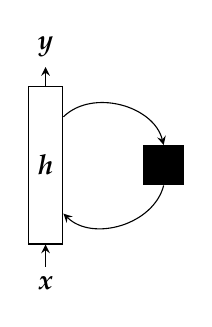
\begin{tikzpicture}[x=1.5cm, y=1.5cm]
      \node [] (input) at (0,0) {$\vect{x}$};

      \node [layer] (state) at (0,1) {$\vect{h}$};
      \node [delay] (delay) at (1,1) {};

      \node [] (output) at (0,2) {$\vect{y}$};
      
      \draw [arrow] (input) -- (state);
      \draw [arrow] (state) -- (output);
      \draw (state) edge[arrow, bend left=60] (delay.north);
      \draw (delay.south) edge[arrow, bend left=60] (state);
    \end{tikzpicture}
  }\hfill
  % \subfigure[]{
  \subfloat[\label{fig:rnn2}]{
    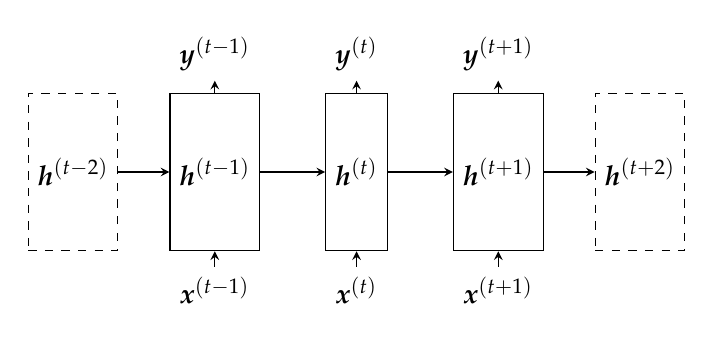
\begin{tikzpicture}[x=1.5cm, y=1.5cm]
      \foreach \l [count=\i] in {t-1,t,t+1}{
        \node [] (input-\i) at (\i*1.2,0) {$\vect{x}^{(\l)}$};
        \node [layer] (state-\i) at (\i*1.2,1) {$\vect{h}^{(\l)}$};
        \node [] (output-\i) at (\i*1.2,2) {$\vect{y}^{(\l)}$};

        \draw [arrow] (input-\i) -- (state-\i);
        \draw [arrow] (state-\i) -- (output-\i);
      }
      \node [layer, dashed] (state-l) at (0,1) {$\vect{h}^{(t-2)}$};
      \node [layer, dashed] (state-r) at (4*1.2,1) {$\vect{h}^{(t+2)}$};

      \draw [arrow] (state-l) -- (state-1);
      \draw [arrow] (state-1) -- (state-2);
      \draw [arrow] (state-2) -- (state-3);
      \draw [arrow] (state-3) -- (state-r);
    \end{tikzpicture}
  }
  \caption{\acf{rnn}, folded (a) and unfolded (b) models.}
  \label{fig:rnn}
\end{figure}
In order to express a compact visualisation of \acp{rnn} it is
possible to use the computational graph in \cref{fig:rnn1} where the
black box is a 
delay of one iteration. An extract of the unfolding of the computation
graph is 
shown in \cref{fig:rnn2}. 

\begin{figure}
  \centering
  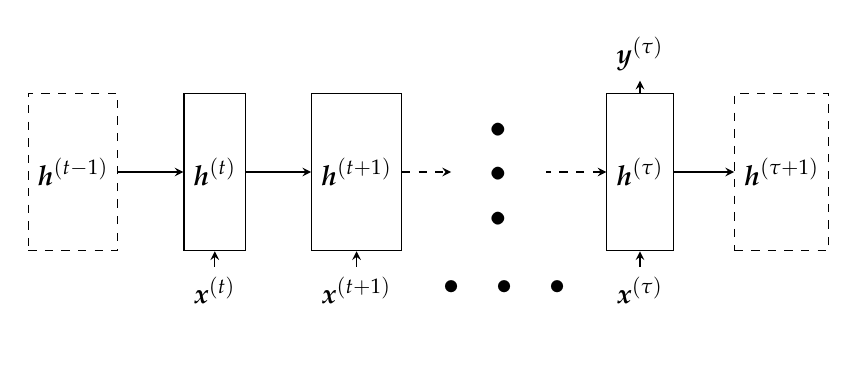
\begin{tikzpicture}[x=1.5cm, y=1.5cm]
    \foreach \l [count=\i] in {t,t+1,missing,\tau}{
      \ifthenelse{\equal{\l}{missing}}{
        \node [vmissing] (state-\i) at (\i*1.2,1) {};
        \node [hmissing] (state-\i) at (\i*1.2,0) {};
      }{
        \node [] (input-\i) at (\i*1.2,0) {$\vect{x}^{(\l)}$};
        \node [layer] (state-\i) at (\i*1.2,1) {$\vect{h}^{(\l)}$};
        \draw [arrow] (input-\i) -- (state-\i);
        \ifthenelse{\equal{\l}{\tau}}{
          \node [] (output-\i) at (\i*1.2,2) {$\vect{y}^{(\l)}$};
          \draw [arrow] (state-\i) -- (output-\i);
        }
      }
    }

    \node [layer, dashed] (state-l) at (0,1) {$\vect{h}^{(t-1)}$};
    \node [layer, dashed] (state-r) at (5*1.2,1) {$\vect{h}^{(\tau+1)}$};

    \draw [arrow] (state-l) -- (state-1);
    \draw [arrow] (state-1) -- (state-2);
    \draw [arrow,dashed] (state-2) -- ++(0.8,0);
    \draw [arrowInverse,dashed] (state-4) -- ++(-0.8,0);
    \draw [arrow] (state-4) -- (state-r);
  \end{tikzpicture}
  \caption{\ac{rnn} with single output after a sequence of inputs.}
  \label{fig:rnnSO}
\end{figure}
The model in \cref{fig:rnn} provides an output $\vect{y}^{(t)}$ for every
input $\vect{x}^{(t)}$. An alternative is the model of
\cref{fig:rnnSO} where an output $\vect{y}^{(\tau)}$ is provided only
after a sequence $\vect{x}^{(t)},\dots,\vect{x}^{(\tau)}$ of inputs.

In order to train a \ac{rnn}, it is sufficient to apply the
backpropagation to the entire unfolded model.

\subsection{\acf{lstm}}
The major drawback of \acp{rnn} is the \emph{vanishing
  gradient} problem during the backpropagation. The gradient
for long-term associations, propagated through many stages, tends to
become zero. A possible solution for this problem is \ac{lstm} \cite{hochreiter_1997_lstm}.

\begin{figure}
  \centering
  % \subfigure[]{
  \subfloat[]{
    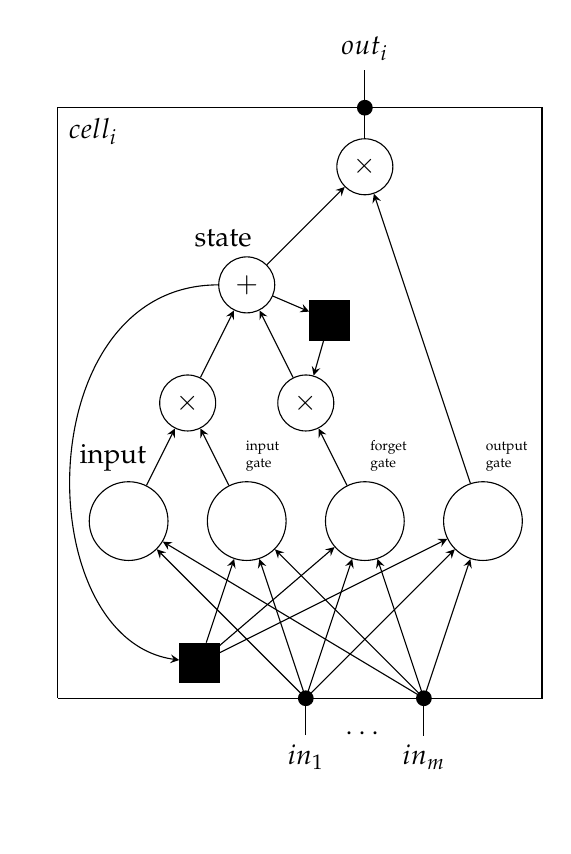
\begin{tikzpicture}[x=1.5cm, y=1.5cm]
      \node at (1,-0.5) {};

      \node[delay] (delay1) at (1.6,0.8) {};
      \coordinate (input1) at (2.5,0.5);
      \coordinate (input2) at (3.5,0.5);
      \node[] (input01) at (2.5,0) {$in_1$};
      \node[] (input02) at (3.5,0) {$in_m$};
      \node[] at (3,0.2) {$\cdots$};
      \node[every neuron, label={[xshift=-2mm]input}] (inputN) at (1,2) {};
      \node[every neuron, label={[xshift=2mm, align=left, font=\tiny] input\\gate}] (inputGate) at (2,2) {};
      \node[every neuron, label={[xshift=3mm, align=left, font=\tiny] forget\\gate}] (forgetGate) at (3,2) {};
      \node[every neuron, label={[xshift=3mm, align=left, font=\tiny] output\\gate}] (outputGate) at (4,2) {};
      \node[operation] (inputTimes) at (1.5, 3) {$\times$};
      \node[operation, label={[xshift=-3mm]state}] (state) at (2, 4) {$+$};
      \node[delay] (delay2) at (2.7,3.7) {};
      \node[operation] (forgetTimes) at (2.5, 3) {$\times$};
      \node[operation] (outputTimes) at (3, 5) {$\times$};
      \coordinate (output1) at (3,5.5);
      \node (output2) at (3,6) {$out_i$};
      \node at (0.7,5.3) {$cell_i$};

      \fill[black] (input1) circle (1mm);
      \fill[black] (input2) circle (1mm);
      \fill[black] (output1) circle (1mm);
      
      \foreach \n in {input1, input2}{
        \foreach \m in {inputN, inputGate, forgetGate, outputGate}{
          \draw[arrow] (\n) -- (\m);
        }
      }
      \foreach \m in {inputGate, forgetGate, outputGate}{
        \draw[arrow] (delay1) -- (\m);
      }

      \draw[arrow] (inputN) -- (inputTimes);
      \draw[arrow] (inputGate) -- (inputTimes);
      \draw[arrow] (forgetGate) -- (forgetTimes);
      \draw[arrow] (inputTimes) -- (state);
      \draw[arrow] (forgetTimes) -- (state);
      \draw [arrow] (state) ..  controls  (0.15,4) and (0.15,1) ..  (delay1);
      \draw[arrow] (state) -- (delay2);
      \draw[arrow] (delay2) -- (forgetTimes);
      \draw[arrow] (state) -- (outputTimes);
      \draw[arrow] (outputGate) -- (outputTimes);
      \draw[line] (outputTimes) -- (output1);
      \draw[line] (output1) -- (output2);
      \draw[line] (input01) -- (input1);
      \draw[line] (input02) -- (input2);

      \path[border] (0.4,0.5) -- (4.5,0.5) -- (4.5,5.5) -- (0.4,5.5) -- (0.4,0.5); 
      

    \end{tikzpicture}
    \label{fig:lstm1}
  }\hfill
  % \subfigure[]{
  \subfloat[]{
    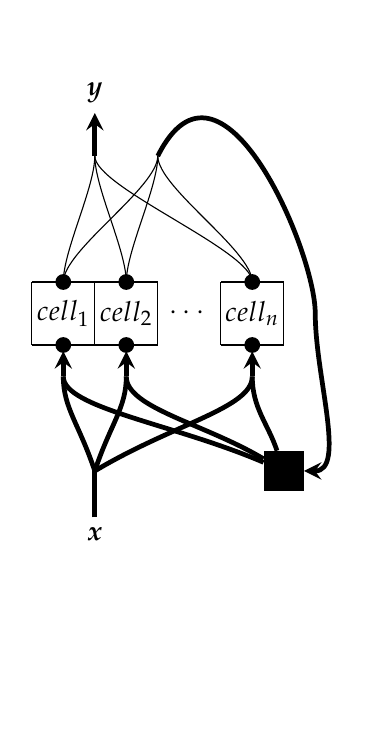
\begin{tikzpicture}[x=0.8cm, y=0.8cm]
      \node at (1,-2.5) {};

      % \draw[step=1.0,black,thin] (0,3) grid (4,4);
      \draw[step=1.0,black,thin] (0,3) grid (2,4);
      \draw[step=1.0,black,thin] (3,3) grid (4,4);
      \coordinate (input1) at (0.5,3);
      \coordinate (input2) at (1.5,3);
      \coordinate (input3) at (3.5,3);
      \coordinate (inputM1) at (0.5,2.5);
      \coordinate (inputM2) at (1.5,2.5);
      \coordinate (inputM3) at (3.5,2.5);
      \coordinate (output1) at (0.5,4);
      \coordinate (output2) at (1.5,4);
      \coordinate (output3) at (3.5,4);

      \coordinate (outputM) at (2,6);
      \coordinate (outputTM) at (1,6);
      
      \node at (0.5, 3.5) {$cell_1$};
      \node at (1.5, 3.5) {$cell_2$};
      \node at (2.5, 3.5) {$\cdots$};
      \node at (3.5, 3.5) {$cell_n$};
      \coordinate (pass) at (4.5, 3.5);
      \node (inputT) at (1,0) {$\vect{x}$};
      \coordinate (inputTM) at (1,1);
      \node (outputT) at (1,7) {$\vect{y}$};

      \node[delay] (delay) at (4,1) {};

      \foreach \c in {input1, input2, input3, output1, output2, output3}{
        \fill[black] (\c) circle (1mm);
      }

      \foreach \c in {inputM1, inputM2, inputM3}{
        \draw [vectorLine] (delay) ..  controls
        ($0.5*(delay)+0.5*(\c)$) and ($(\c)-(0,0.5)$) ..  (\c);
        \draw [vectorLine] (inputTM) ..  controls
        ($0.5*(inputTM)+0.5*(\c)$) and ($(\c)-(0,0.5)$) ..  (\c);
      }

      \foreach \c in {1, 2, 3}{
        \draw[vectorArrow] (inputM\c) -- ($(input\c)-(0,0.1)$);
      }

      \foreach \c in {output1, output2, output3}{
        \draw [line] (\c) ..  controls  ($(\c)+(0,0.5)$) and
        ($(outputM)-(0,0.5)$) ..  (outputM);
        \draw [line] (\c) ..  controls  ($(\c)+(0,0.5)$) and
        ($(outputTM)-(0,0.5)$) ..  (outputTM);
      }

      %\draw [vectorArrow] (outputM) ..  controls  ($(outputM)+(1,2)$) and ($(delay)+(1,0)$) ..  (delay);
      \draw [vectorArrow]
      (outputM) ..
      controls  ($(outputM)+(1,2)$) and ($(pass)+(0,1)$) ..
      (pass) ..
      controls  ($(pass)-(0,1)$) and ($(delay)+(1,0)$) ..
      (delay);
      \draw[vectorLine] (inputT) -- (inputTM);
      \draw[vectorArrow] (outputTM) -- (outputT);
    \end{tikzpicture}
    \label{fig:lstm2}
  }
  \caption{\ac{lstm} model: detail of memory cell (a), and general
    scheme (b). The black box is a delay of one iteration.}
  \label{fig:lstm}
\end{figure}
The \ac{lstm} model is structured as in \cref{fig:lstm}. It is
equivalent to a
generic \ac{rnn} where the hidden state $\vect{h}$ is a
layer of \emph{memory cells}.

In detail a single
memory cell (\cref{fig:lstm1}) has four \acf{an}. One is labelled \emph{input}
and processes the cell's 
inputs into an internal state. The other three \ac{an} are labelled as
\emph{gates} and process the cell's inputs together with the previous-phase
state in order to decide:
\begin{itemize}
\item how much of the current input must be learned
  (\emph{input gate});
\item how much of the previous-phase state must be forgotten
  (\emph{forget gate});
\item how much of the state constitutes the output (\emph{output gate}).
\end{itemize}

The memory-cells layer (\cref{fig:lstm2}) is composed of a number of
cells equal to the dimension of the output. Each cell
calculates one dimension of $\vect{y}$. The input $\vect{x}$ is copied
for every cell and, together with the previous-phase
output,
constitutes the input $in_1,\dots,in_m$ of the single cells.

\section{metrics}
We used different metrics in order to evaluate the models.
All the metrics are defined between $0$ and $1$ or between $-1$ and $1$,
higher is the value, better is the assessment.

\subsection{Accuracy}
is defined
as the ratio between the correct-classified and all documents. If $\vect{y}$
is the ground truth and $\vect{\hat y}$ is the predicted
classification vectors for $n$ samples, then the accuracy is defined
as:
\begin{equation*}
  accuracy\left(\vect{y}, \vect{\hat y}\right) \equiv
  \frac{1}{n}\sum_{i=1}^{n} 1\left(\hat y_i = y_i\right),
\end{equation*}
Where
\begin{equation*}
  1(a = b)\equiv
  \begin{cases}
    1 & \text{if }a = b,\\
    0 & \text{otherwise}.
  \end{cases}
\end{equation*}

In an
unbalanced dataset, like the one of this work, it is a biased score -
a model that predicts well only the most frequent classes, and ignore
the rest, achieve a good accuracy. To resolve this we considered also
other metrics.

\subsection{Cohen's kappa} score is usually used to asses
the agreement of two annotators \cite{cohen_coefficient_1960}. It
measures the difference between the observed agreement and the
agreement that can happen by choosing randomly the class. It can then
be used to mitigate the bias caused by the unbalanced dataset. Cohen's
kappa is defined as:
\begin{equation*}
  \kappa(\vect{y}, \vect{\hat y})\equiv \frac{p_o(\vect{y}, \vect{\hat y}) -p_e(\vect{y}, \vect{\hat y})}{1-p_e(\vect{y}, \vect{\hat y})} = 1-\frac{1-p_o(\vect{y}, \vect{\hat y})}{1-p_e(\vect{y}, \vect{\hat y})},
\end{equation*}
where $p_o$ is the observed agreement that is equal to the accuracy
and $p_e$ represents the probability of agreement by chance. For $n$
samples and $k$ classes it is
defined by:
\begin{equation*}
  p_e(\vect{y}, \vect{\hat y}) = \frac{1}{n^2}\sum_{i=1}^{k} \mu_{i}(\vect{y})\cdot\nu_{i}(\vect{\hat y}),
\end{equation*}
where $\mu_{i}$ and $\nu_{i}$ are the number of samples classified as
$i$ for the first and second classifier. They are defined as:
\begin{eqnarray*}
  \mu_i(\vect{y}) &=& \sum_{j=1}^{n}1(y_j = i)\\
  \nu_i(\vect{\hat y}) &=& \sum_{j=1}^{n}1(\hat y_j = i)
\end{eqnarray*}

\subsection{\acf{map}} is a measure used in information
retrieval. It expresses how well the true classification can be retrieved in
the first results of the classifier. We define two variants of
\ac{map}, one (MAPc) to state how well all records for a specific class are
retrieved, the other (MAPs) to asses how well the correct class is retrieved
for a specific sample. The first is defined for $n$ samples and $k$ classes,
with $\vect{Y}=\vect{y}_1,\dots,\vect{y}_k$ and $\vect{\hat
  Y}=\vect{\hat y}_1,\dots,\vect{\hat y}_k$ the ground truth and
prediction $n\times k$ matrices. The formula is:
\begin{equation*}
  MAPc(\vect{Y}, \vect{\hat Y})\equiv
  \frac{1}{k}\sum_{c=1}^{k}AveP(\vect{y}_c, \vect{\hat y}_c),
\end{equation*}
where $AveP$ is the average precision for class $c$:
\begin{equation*}
  AveP(\vect{y}, \vect{\hat y}) \equiv
  \frac{1}{\sum_{i=1}^k 1(y_i)}\sum_{j=1}^k P_j(\vect{y}, \vect{\hat y})\cdot 1(y_{\sigma_{\vect{\hat y}}(j)}),
\end{equation*}
where $1(y)$ is an indicator
function that is $1$ for the elements classified positively, $0$
otherwise. $\sigma_{\vect{\hat y}}(j)$ is a function that returns the
  index in $\vect{\hat y}$ of the $j$-th element in the ordered
  version of $\vect{\hat y}$ . $P_j$ is defined as:
\begin{equation*}
P_j(\vect{y}, \vect{\hat y}) \equiv \frac{1}{j}\sum_{c=1}^j
1(y_{\sigma_{\vect{\hat y}}(c)}).
\end{equation*}

MAPs is defined like MAPc, but on the transposed classification
matrices
\begin{equation*}
  MAPs(\vect{Y}, \vect{\hat Y})\equiv
  MAPc(\vect{Y}^T, \vect{\hat Y}^T)
\end{equation*}

\subsection{Precision} is defined for $n$ samples and binary
classifications as:
\begin{equation}\label{eq:precision}
P(\vect{y}, \vect{\hat y}) \equiv \frac{\sum_{s=1}^n 1(\hat
  y_s \text{ and }y_s)}{\sum_{s=1}^n 1(\hat y_s)}.
\end{equation}
It expresses the ratio of correct positive predictions over all the
positive predictions.

\subsection{Recall} conversely, is defined as:
\begin{equation}\label{eq:recall}
R(\vect{y}, \vect{\hat y}) \equiv \frac{\sum_{s=1}^n 1(\hat
  y_s \text{ and }y_s)}{\sum_{s=1}^n 1(y_s)},
\end{equation}
and it is the ratio of correct predicted positive over all the positive
classes.

\subsection{F1-score} is the harmonic mean of precision and recall,
combining the two measures:
\begin{equation*}
F_1(\vect{y}, \vect{\hat y}) \equiv 
2\frac{P(\vect{y}, \vect{\hat y})\cdot R(\vect{y}, \vect{\hat y})}
{P(\vect{y}, \vect{\hat y})+R(\vect{y}, \vect{\hat y})}.
\end{equation*}

Precision, recall, and thus $F_1$ score are defined only for binary
classifiers. In order to use those metrics in a multi-class
classification problem it is possible to average the measures for the
different classes. We considered different methodologies of averaging:
\begin{description}
  \item[micro] averaging is performed flattening the array of truth
    and prediction of the different classes and then appling the
    scoring formula;
  \item[macro] average is performed calculating the metrics on the
    single classes and then averaging them:
    \begin{equation*}
      \frac{1}{k}\sum_{c=1}^k S(\vect{y}_c, \vect{\hat y}_c);
    \end{equation*}
  \item[weighted] average uses the normalized number of samples for
    each class in order to give a weight to them:
    \begin{equation*}
      \frac{1}{\sum_{i=1}^k|\vect{\hat y}_i|}\sum_{c=1}^k|\vect{\hat y}_c|\cdot S(\vect{y}_c, \vect{\hat y}_c).
    \end{equation*}
\end{description}

Micro average considers all the samples equally, regardless of the
representativeness of classes in the dataset. Macro average takes
into account the unbalancement and it is more sensible to few
represented classes. Precision, recall, and $F_1$ score are
equal to the accuracy when micro averaged in a multiclass
environment. 

\subsection{ROC curve} is a graph of \emph{true positive rate} versus
\emph{false positive rate} with the change of the classifier threshold. The
true positive rate is equal to the recall defined in
\cref{eq:recall}. Conversely the false positive rate is defined as:
\begin{equation}\label{eq:fpr}
FPR(\vect{y}, \vect{\hat y}) \equiv \frac{\sum_{s=1}^n 1(\hat
  y_s \text{ and not }y_s)}{\sum_{s=1}^n 1(\text{not }y_s)}.
\end{equation}

ROC curves start from $(0,0)$ and end in $(1,1)$. The area under
the curve can be used as a metric for the classifier, a perfect
classifier has an area of $1$.

The curves can be calculated only for binary classifiers. Like for the
precision, recall and $F_1$ score, it is possible to generalise them to
multiclass problems averaging micro or macro.

\subsection{Precision-recall curve} is a graph of precision
(\cref{eq:precision}) versus 
recall (\cref{eq:recall}) with the change of the classifier
threshold. The curves start from $(0,1)$ and end in $(1,0)$. A perfect
classifier has an area under the curve of $1$.

Also precision-recall curves can be calculated only for binary
classifiers. In order to generalise them to multiclass problem it is
necessary to micro or macro average.




%%% Local Variables:
%%% mode: latex
%%% TeX-master: "thesis"
%%% End:

\chapter{Background}
\label{ch:background}

\section{Text Classification}

\section{Attention models}
Attention models are an important concept in neural networks that has
been researched within diverse application domains.

\section{Existing works on \ac{icdo}}
Early works for ICD-O3 code assignment were based on rule-based
systems, where the code was assigned by creating a set of handcrafted
text search queries and combining results by standard Boolean
operators~\cite{crocetti_automatic_2004}. In order to prevent spurious
matches, rules need to be very specific, making it very difficult to
achieve a sufficiently high recall on future (unseen) cases.

A number of studies reporting on the application of machine learning
to this problem have been published during the last decade. Direct
comparisons among these works are impossible due to the (not
surprising) lack of a standard publicly available dataset and
heterogeneous details in the settings. Still, we highlight in the
following the main differences among them in order to provide some
background. In~\cite{jouhet_automated_2011}, the authors employed
support vector machine (SVM) and Naive Bayes classifiers on a small
dataset of $5\,121$ French pathology reports and a reduced number of
target classes (26 topographic classes and 18 morphological classes),
reporting an accuracy of 72.6\% on topography and 86.4\% on morphology
with SVM. A much larger dataset of $56\,426$ English reports from the
Kentucky Cancer Registry was later employed
in~\cite{kavuluru_automatic_2013}, where linear classifiers (SVM,
Naive Bayes, and logistic regression) were also compared but only on
the topography task and using 14, 42, and 57 classes. The authors
reported a micro-averaged F1 measure of 90\% when using SVM with both
unigrams and bigrams. Still, the bag-of-words representations used by
these linear classifiers do not take word order into account and are
unable to capture similarities and relations among words (which are
all represented by orthogonal vectors). Deep learning techniques are
known to overcome these limitations but were not employed to this
problem until very recently. In~\cite{qiu_deep_2018}, a convolutional
neural network (CNN) architecture fed by word vectors pretrained on
PubMed was applied to a small corpus of 942 breast and lung cancer
English reports with 12 topography classes; the authors demonstrate
the superiority of this approach compared to linear classifiers with
significant increases in both micro and macro F1
measure. In~\cite{gao_hierarchical_2018}, the same research group also
experimented on the same dataset using recurrent neural networks (RNN)
with hierarchical attention~\cite{yang_hierarchical_2016}, obtaining
further improvements over the CNN architecture.

%%% Local Variables:
%%% mode: latex
%%% TeX-master: "thesis"
%%% End:

\chapter{\ac{icdo} classification}
\label{ch:icdo}

\section{Dataset}
We collected a set of $1\,592\,385$ anatomopathological exam results
from Tuscany region in the period 2004-2013. About $6\%$
of these records refer to a positive tumor
diagnosis and have topological and morphological ICD-O3 labels,
determined by tumor registry experts. Other reports are associated
with non-cancerous tissues and with unlabeled records. When multiple
pathological records for the
same patient existed for the same tumor, experts selected the most
informative report in order to assign the ICD-O3 code to that tumor
case, leaving a set of $94\,524$ labeled tumor cases.

Histological exam records consist of three free-text fields (not all
of them always filled-in), reporting tissue macroscopy, diagnosis,
and, in some cases, the patient's anamnesis. We found that field
semantics was not always used consistently and that the amount of
provided details varied significantly from extremely synthetic to very
detailed assessments of the morphology and the diagnosis. Field length
ranged from $0$ to $1\,368$ words, with first quartile, median and
third quartile respectively 34, 62, 134. For these reasons we merged
the three text fields
into a single text document, did not apply any conflation (except for
case normalization) kept punctuation. We finally removed duplicate
reports and reports labeled with extremely rare (1048
samples that not
appear in either training, validation, and test sets) ICD-O3 codes. We
obtained in the end 
a dataset suitable for supervised learning consisting of $85\,170$
labeled records over $203$ morphological classes and $68$
topological classes (see below).

\section{Prediction tasks}
A topographical \ac{icdo3} code is structured as \emph{Cmm.s} where
\emph{mm} and \emph{s} represent the main site and the subsite,
respectively. For example, \emph{C50.2}
is the code for the upper-inner quadrant (\emph{2}) of breast (\emph{50}).

A morphological \ac{icdo3} code is structured as \emph{tttt/b}
where \emph{tttt} and \emph{b} represent the cell type and the tumor
behavior (benign, uncertain, in-situ, malignant primary site,
malignant metastatic site), respectively. For example, \emph{8140/3}
is the code for an adenocarcinoma (\emph{adeno 8140};
\emph{carcinoma 3}).

We defined two multi-class classification tasks: (1) main tumor site
prediction ($68$ mutually exclusive classes) and (2) morphology
prediction ($203$ mutually exclusive
classes). Although the two tasks maybe somewhat correlated, we did not
attempt multi-task approaches given the small number of tasks and
large enough size of the dataset.

As shown in \cref{fig:classDist}, the dataset is highly unbalanced.
\begin{figure}
  \centering
  \includegraphics[width=\floatwidth]{img/classDist-icdo3-site.pdf}
  \caption{Documents in classes (ordered by
    frequency).}
  \label{fig:classDist}
\end{figure}

\subsection{Recurrent Neural Networks}
\label{sec:rnn}
In our setting, a dataset $\mathcal{D}=\{(\vect{x}^{(i)},y^{(i)})\}$
consists of variable length sequence vectors $\vect{x}^{(i)}$, where
$x^{(i)}_t$, for $t=1,\dots,T^{(i)}$ is the $t$-th word in the $i$-th
document, and associated target classes
$y^{(i)}\in\{1,\dots,K\}$. Unless necessary, we will drop the
superscript in the following to keep notation simple.  Sequences will
be denoted in boldface. The RNN-based sequence classifiers used in
this work compute their predictions $f(\vect{x})$ as follows:
\begin{align}
  e_t &=& E(\vect{x};\theta^e),\label{eq:embed}\\
  h^f_t &=& F(e_t,h^f_{t-1};\theta^f),\label{eq:maxModelRL}\\  
  h^b_t &=& R(e_t,h^r_{t+1};\theta^r),\label{eq:maxModelRR}\\
  u_t &=& G(h_t;\theta^h),\label{eq:maxModelF}\\
  \phi & =& A(\vect{h},\vect{u};\theta^a),\label{eq:aggregation}\\
  f(\vect{x}) &=& g(\phi;\theta^c).\label{eq:maxModelC}
\end{align}
$E$ is an embedding function mapping words into $p$-dimensional real
vectors (where embedding parameters $\theta_e$ can be either
pretrained and adjustable or fixed, see Section~\ref{sec:word-vectors}
below.  Functions $F$ and $R$ corresponds to (forward and reverse)
dynamics that can be described in term of several (possibly layered)
recurrent cells. In this work we focus on gated recurrent unit (GRU)
cells~\cite{cho2014properties} for their simplicity and because
preliminary experiments revealed no advantages over long-short term
memory cells~\cite{hochreiter1997long} on our data. Each vector $h_t$,
the concatenation of $h^l_t$ and $h^r_t$, can be interpreted as latent
representations of the information contained at position $t$ in the
document. $G$ is an additional layer mapping each latent vector into a
vector $u_t$ that can be seen as contextualized representation of the
word at position $t$. $A$ is an aggregation function that creates a
single $d$-dimensional representation vector for the entire sequence
and $g$ is a softmax layer. Possible choices for the aggregator
function include:
\begin{itemize}
\item $\phi=(h^f_T,h^r_1)$, which just
  extract the extreme latent representations; these may be in
  principle sufficient since they depend on the whole sequence due to
  bidirectional dynamics; note however that this approach may require
  long-term dependencies to be effectively learned.
\item
  $\phi = \sum_t a_t(\vect{u};\theta^a) h_t$,
  using an attention mechanism as in~\cite{yang_hierarchical_2016}; in
  this case, (scalar) attention weights are computed as
  $$
  a_t(\vect{u};\theta^a) = \frac{e^{\langle \theta^a, u_t\rangle}}
  {\sum_s{e^{\langle \theta^a, u_s\rangle}}}
  $$
\item $\phi = \max_t u_t$ where the maximum is taken element-wise
  along the sequence; this approach can be interpreted either as a
  simplified (parameter-less) attention mechanism or a bag-layer as
  proposed in the context of multi-instance
  learning~\cite{tibo2017network}; in this case each ``feature''
  $\phi_j$ will be positive if at least one of $u_{j,1},\dots,u_{j,T}$
  is positive; the resulting classifier will find it easy to create
  decision rules predicting a document as belonging to a certain class
  if a given set of contextualized word representations are present
  and another given set of contextualized word representations are
  absent in the sequence.
\end{itemize}

The parameters $\theta^f,\theta^r,\theta^h$ and $\theta^a$ (if
present) are determined by minimizing a loss function $\loss$
(categorical cross-entropy in our case) on training data:
\begin{equation}
  \hat \theta = \mathrm{arg}\min_\theta\sum_{(\vect{x},y)\in\mathcal{D}}\loss\left(y,f(\vect{x})\right).
\end{equation}


\section{Baseline}

\subsubsection{Linear classifiers}
The classic approach is to employ bag-of-words
representations of textual documents.
%In this approach, a document is 
%described by a \textit{set} or a \textit{multiset} of words.
%Multisets allow one to take into account the number of occurrences of
%a word in the document.
Vector representations of documents are easily
derived from bags-of-words either by using indicator vectors or taking
into account the number of occurrences of each word using the
\ac{tfidf}\cite{manning_introduction_2008}. In those representations,
frequent and non-specific terms receive a lower weight.

Bag-of-words representations (including those employing bigrams or
trigrams) enable the application of very simple text classifiers such
as \ac{nb} or \ac{svm} \cite{cortes-support-1995}, but they
suffer two fundamental problems. First, the relative order of terms in
the documents is lost, making it impossible to take advantage of the
syntactic structure of the sentences. Second, distinct words have an
orthogonal representation even when they are semantically
close. As detailed in the next section, word vectors can be used to
address the second limitation and also allow us to take advantage of
unlabeled data, which can be typically be obtained in large amounts
and with little cost.

\subsubsection{\acs{bert}}
\ac{bert} \cite{devlin2018bert} is a recent model that represents the
state of the art in many \ac{nlp} related tasks
\cite{chatterjee2019semeval,hu2019introductory,lee2019biobert,tshitoyan2019unsupervised}.
It is a
bi-directional pre-training model backboned by the Transformer Encoder
\cite{vaswani2017attention}. It is an attention-based technique that
learns context-dependent word representation on large unlabeled
corpora, and then the model is fine tuned end to end on specific labeled
tasks. During pre-training, the model is trained
on unlabeled data over two different tasks. In \ac{mlm} some tokens
are masked and the model is trained to predict those token based on
the context. In \ac{nsp} the model is trained to understand the
relationship between sentences predicting if two sentences are actually
consecutive or if they where randomly replaced (with 50\%
probability). After the pre-training, the model is fine-tuned to the
specific task.


\subsection{Hyperparameters}
The hyperparameters $\xi=\xi^l\cup\xi^r\cup\xi^h\cup\xi^c$ define the
structure of the model. Regarding $\xi^l=\xi^r$ they define the type
of \ac{rnn} that in our experiments can be \ac{lstm} or \ac{gru}, the
number of stacked \ac{rnn} layers and the dimension of each
layer. $\xi^h$ defines the number of layers in the first
\ac{mlp} and their
dimensions, moreover it defines the type of aggregating function $f$
that in our experiments can be one of
\begin{align}
  f(\vect{a},\vect{b}) &= \left[\max(a_1,b_1),\dots,\max(a_l,b_l)\right];\\
  f(\vect{a},\vect{b}) &= \left[\frac{a_1+b_1}{2},\dots,\frac{a_l+b_l}{2}\right];\\
  f(\vect{a},\vect{b}) &= \left[a_1,\dots,a_l,b_1,\dots,b_l\right].\label{eq:aggregation}
\end{align}
$\xi^c$ defines the number of layers and their dimensions of the
final classifier. The number of layers defined in $\xi^h$ can be
equal to $0$. In such case, $\vect{h}_{i,j}$ is calculated:
\begin{equation*}
  \vect{h}_{i,j} = f(\vect{h}^l_{i,j},\vect{h}^r_{i,j}).
\end{equation*}
Also the number of layers defined in $\xi^c$ can be equal to $0$. In
such case $\vect{\hat{y}}_i$ is calculated:
\begin{equation*}
  \vect{\hat y}_i = \max_j(\vect{h}_{i,j}).
\end{equation*}

\section{Results}
\subsection{Artificial dataset}\label{sec:experiments}
Classic \ac{rnn} approaches exhibit some limits related to
memory. We designed an artificial experiment in
order to investigate how \ac{rnn} and \ac{max} address those
problems. The dataset 
$D=(\vect{X}\in [0,\dots,9]^{n\times m},\vect{y}\in [0,1]^n)$ is
composed of $n$ sequences of length
$m$ of digits $x_{i,j}\in[0,\dots,9]$. If the $i$-th sequence contains
at least three consecutive digits
$x_{i,j-1},x_{i,j},x_{i,j+1}$ that concatenated represents a prime
number then the
sample is positive and labeled with $y_i=1$, otherwise is negative and
$y_i=0$.

We realized a series
$D^{(m)}=(\vect{X}^{(m)},\vect{y}^{(m)})$ of balanced
datasets of increasing complexity. Each $D^{(m)}$ has $100\ 000$
samples with 
sequence lengths of $m\in
[100,200,300,400,500,600,700,800,900,1000]$. We trained two models on
all the datasets: a plain \ac{gru} with hidden dimension $32$ and a
\ac{max} with same hidden dimension $32$. 

\begin{figure}
  \centering
  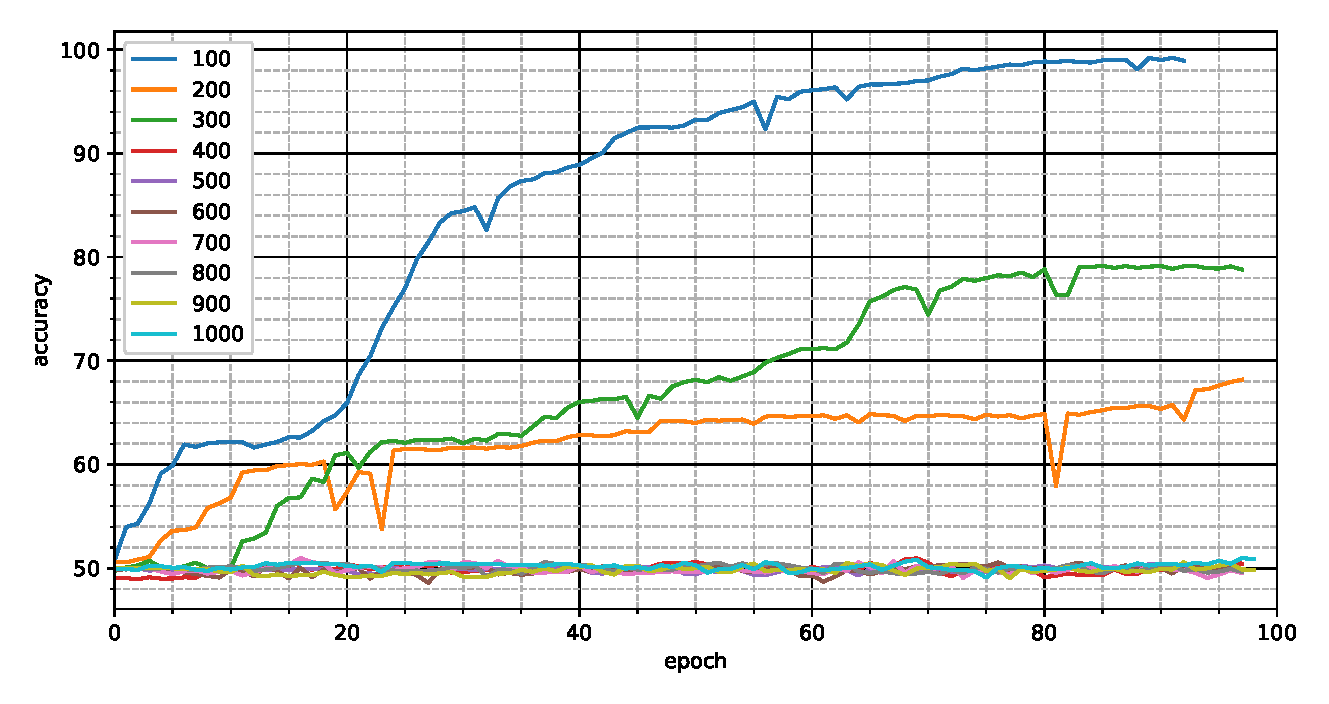
\includegraphics[width=\floatwidth]{imgMax/accuracy-base.eps}
  \caption{Accuracy of plain \ac{gru} on $D^{(m)}$ for different dimensions of $m$.}
  \label{fig:testAccBase}
\end{figure}

\begin{figure}
  \centering
  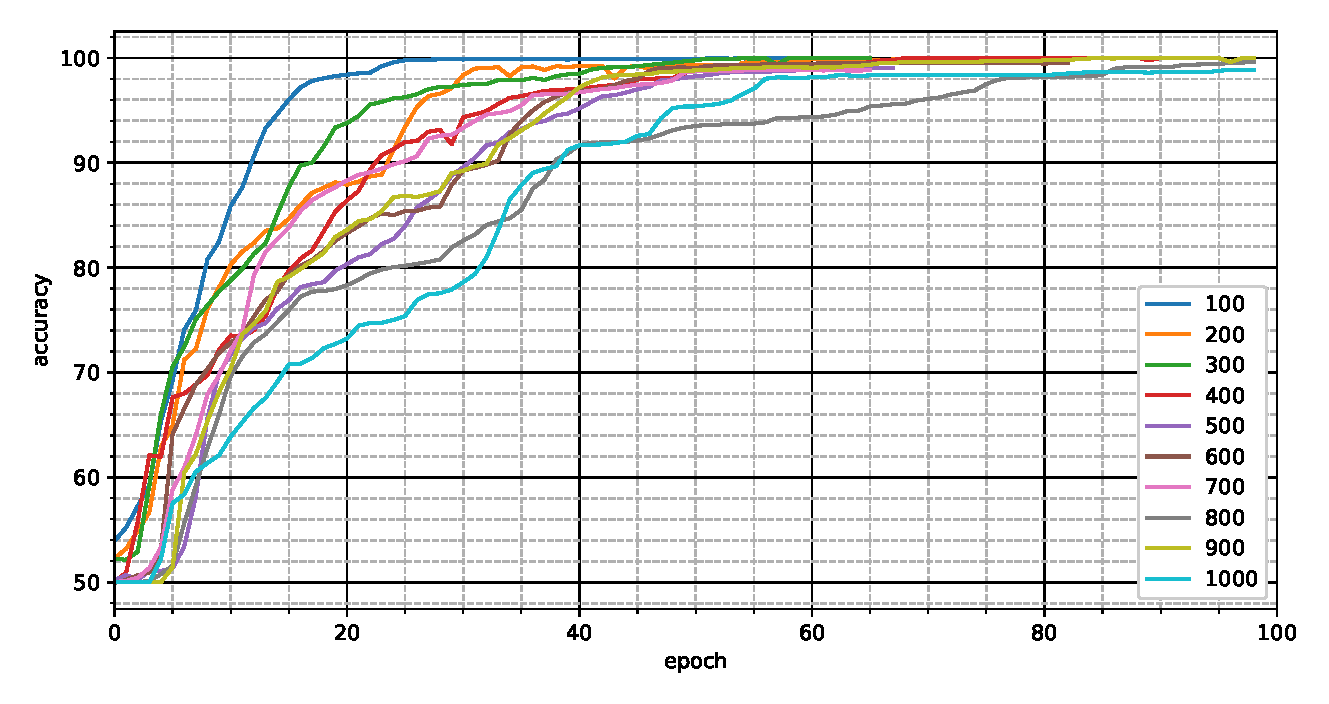
\includegraphics[width=\floatwidth]{imgMax/accuracy-max.eps}
  \caption{Accuracy of \ac{max} on $D^{(m)}$ for different dimensions of $m$.}
  \label{fig:testAccMax}
\end{figure}

In \cref{fig:testAccBase} and \cref{fig:testAccMax} we compare
the learning curves of the base model with \ac{max}. The \ac{gru}
model degrades rapidly respect \ac{max}, under the assumption of
having the same number of parameters.

\subsection{Interpretability}
\ac{max} is flexible enough to gain interpretability under certain
assumptions. Setting in $\xi^c$ in \eqref{eq:maxModelC} the number of
layers to 0 implies that 
the dimension of the last layer in $\xi^h$ in \eqref{eq:maxModelF}
needs to be equal to the
output dimension. We hypothesize that in this setting, the values of
$\vect{h}_{i,j}$ collect information on the importance of the area
around $x_{i,j}$ for the purpose of classification task. This
information can be
used to interpret the model decision. To validate the
hypothesis we performed the same experiment of \cref{sec:experiments}
with an interpretable model with a comparable number of parameters. We
set to 0 the number of layers in \eqref{eq:maxModelC} and to 1 with an
output dimension of 1  in
\eqref{eq:maxModelF}. 

\begin{figure}
  \centering
  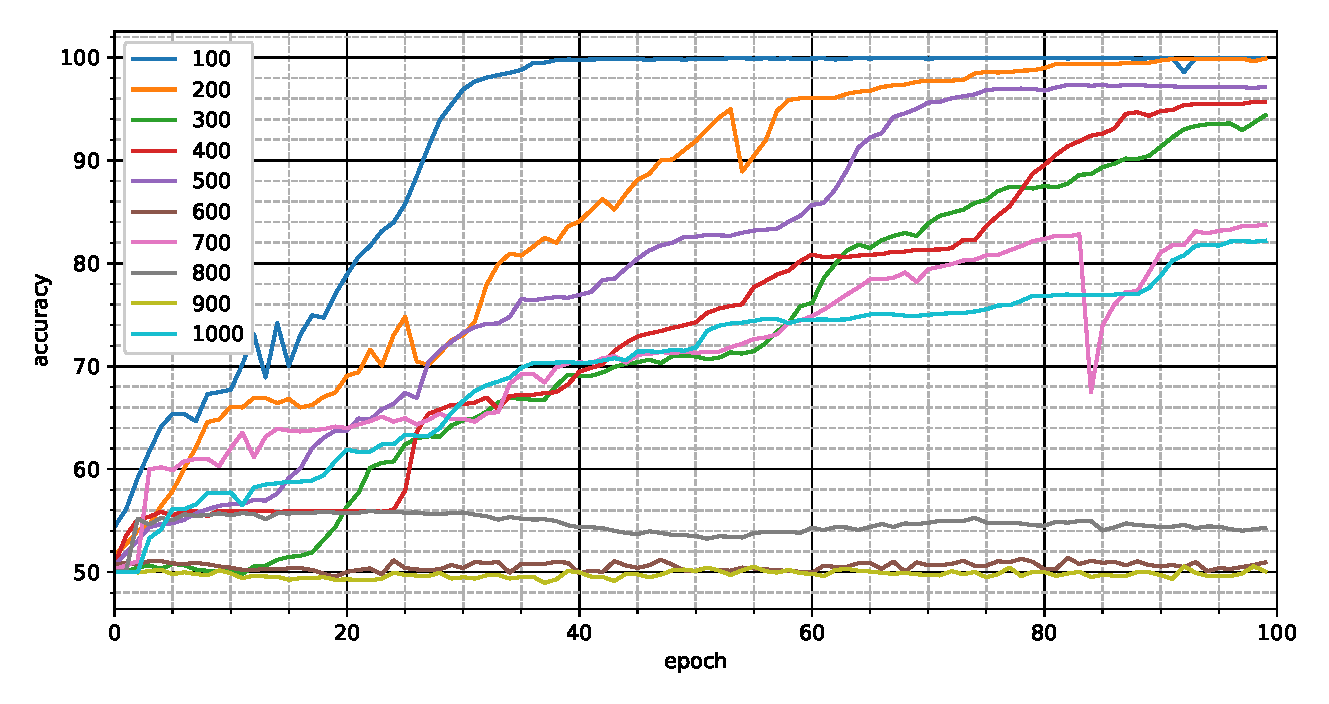
\includegraphics[width=\floatwidth]{imgMax/accuracy-int.eps}
  \caption{Accuracy of interpretable \ac{max} on $D^{(m)}$ for different dimensions of $m$.}
  \label{fig:testAccInt}
\end{figure}
\begin{figure}
  \centering
  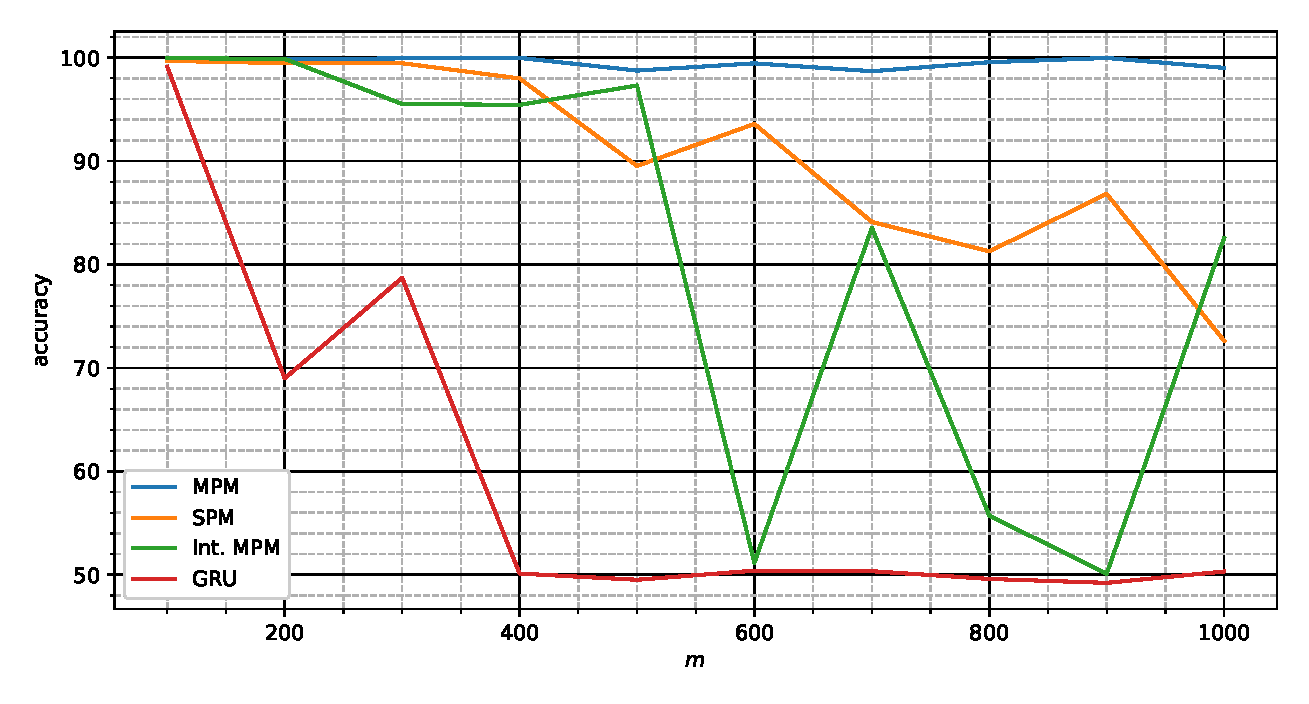
\includegraphics[width=\floatwidth]{imgMax/maxBaseDiff.eps}
  \caption{Max reached accuracy of \ac{max} and \ac{gru} models on $D^{(m)}$ for different dimensions of $m$.}
  \label{fig:testAccDiff}
\end{figure}
\begin{figure}
  \centering
  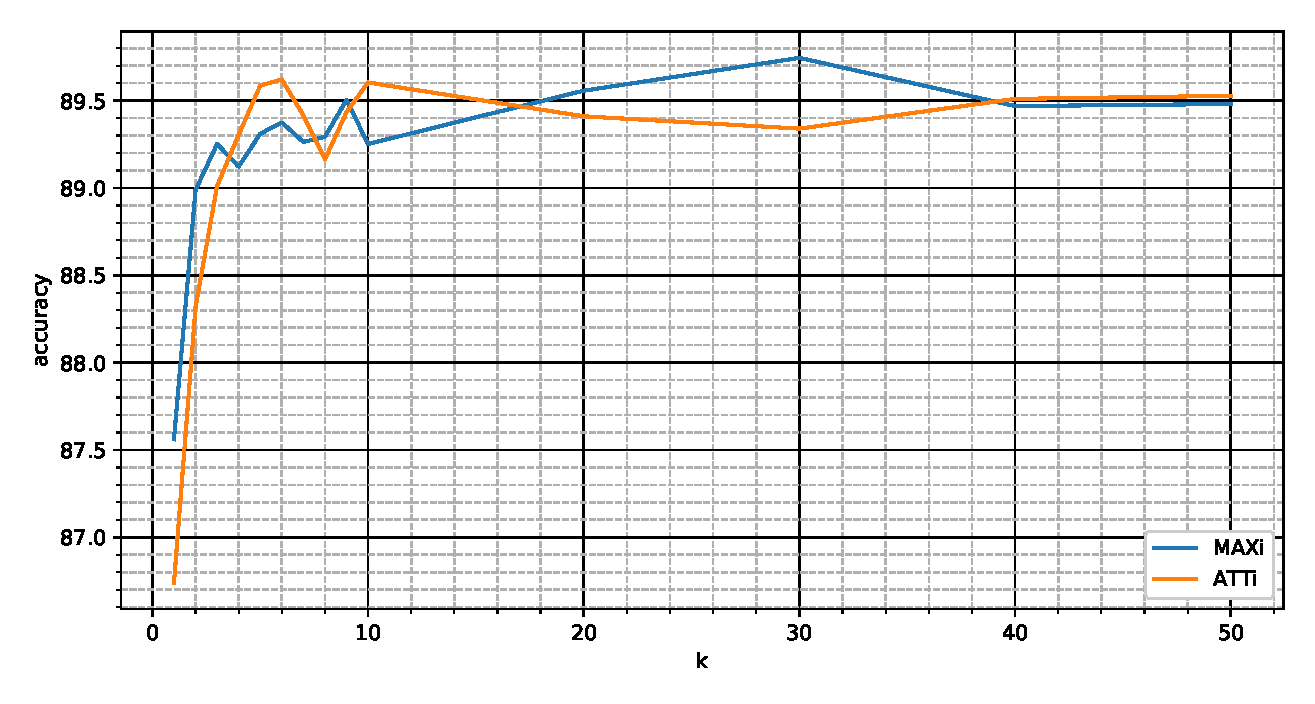
\includegraphics[width=\floatwidth]{img/plotSintex.eps}
  \caption{.}
  \label{fig:sintex}
\end{figure}

\begin{figure}
  \centering
  \footnotesize
  \begin{tabular}{|p{\floatwidth}|}
    \hline
    \input{attentions/test1.tex}\\
    \hline
    \input{attentions/test2.tex}\\
    \hline
    \input{attentions/test3.tex}\\
    \hline
    \input{attentions/test4.tex}\\
    \hline
    \attvisB{0}{5}{0} \attvisB{3}{5}{0} \attvisB{3}{5}{100} \attvisB{9}{6}{100} \attvisB{7}{100}{100} \attvisB{3}{5}{0} \attvisB{6}{5}{0} \attvisB{8}{6}{0} \attvisB{6}{5}{0} \attvisB{2}{7}{0} \attvisB{1}{6}{0} \attvisB{5}{5}{0} \attvisB{2}{5}{0} \attvisB{4}{5}{0} \attvisB{3}{5}{0} \attvisB{8}{6}{0} \attvisB{4}{7}{0} \attvisB{7}{6}{0} \attvisB{2}{6}{0} \attvisB{1}{7}{0} \attvisB{7}{7}{0} \attvisB{2}{5}{0} \attvisB{9}{6}{0} \attvisB{2}{5}{0} \attvisB{3}{5}{0} \attvisB{1}{6}{0} \attvisB{6}{5}{0} \attvisB{0}{6}{0} \attvisB{0}{6}{0} \attvisB{7}{6}{0} \attvisB{2}{6}{0} \attvisB{0}{5}{0} \attvisB{1}{6}{0} \attvisB{4}{5}{0} \attvisB{3}{5}{0} \attvisB{2}{6}{0} \attvisB{0}{5}{0} \attvisB{9}{6}{0} \attvisB{4}{6}{0} \attvisB{3}{5}{0} \attvisB{6}{4}{0} \attvisB{8}{5}{0} \attvisB{8}{5}{0} \attvisB{0}{6}{0} \attvisB{6}{5}{0} \attvisB{1}{6}{0} \attvisB{2}{5}{0} \attvisB{2}{5}{0} \attvisB{6}{5}{0} \attvisB{7}{7}{0} \attvisB{2}{5}{0} \attvisB{6}{4}{0} \attvisB{5}{5}{0} \attvisB{6}{4}{0} \attvisB{6}{5}{0} \attvisB{4}{6}{0} \attvisB{5}{5}{0} \attvisB{5}{5}{0} \attvisB{2}{5}{0} \attvisB{2}{5}{0} \attvisB{2}{6}{0} \attvisB{1}{6}{0} \attvisB{2}{5}{0} \attvisB{3}{6}{0} \attvisB{7}{7}{0} \attvisB{1}{7}{0} \attvisB{8}{5}{0} \attvisB{8}{5}{0} \attvisB{8}{5}{0} \attvisB{2}{5}{0} \attvisB{8}{5}{0} \attvisB{5}{4}{0} \attvisB{8}{5}{0} \attvisB{3}{5}{0} \attvisB{4}{6}{0} \attvisB{8}{5}{0} \attvisB{5}{5}{0} \attvisB{6}{4}{0} \attvisB{8}{6}{0} \attvisB{0}{5}{0} \attvisB{3}{5}{0} \attvisB{6}{4}{0} \attvisB{9}{6}{0} \attvisB{0}{6}{0} \attvisB{6}{4}{0} \attvisB{0}{5}{0} \attvisB{4}{5}{0} \attvisB{0}{5}{0} \attvisB{8}{5}{0} \attvisB{2}{5}{0} \attvisB{4}{6}{0} \attvisB{5}{5}{0} \attvisB{5}{5}{0} \attvisB{2}{5}{0} \attvisB{4}{5}{0} \attvisB{0}{5}{0} \attvisB{8}{5}{0} \attvisB{3}{5}{0} \attvisB{0}{5}{0} \attvisB{8}{5}{0}
\\
    \hline
    \input{attentions/test6.tex}\\
    \hline
  \end{tabular}
  \caption{Visualization of outputs prior to the max pooling for some
    samples. Red boxes represent the prime numbers ground
    truth, green highlighting represents the values of $h_{i,j}$ in
    \eqref{eq:maxModelF}.}
  \label{fig:testAttention}
\end{figure}

\begin{figure}
  \centering
  \footnotesize
  \begin{tabular}{|p{\floatwidth}|}
    \hline
    \attvisB{3}{0}{0} \attvisB{6}{0}{0} \attvisB{2}{0}{0} \attvisB{9}{0}{0} \attvisB{4}{0}{0} \attvisB{8}{0}{0} \attvisB{0}{0}{0} \attvisB{6}{0}{0} \attvisB{3}{0}{0} \attvisB{0}{0}{0} \attvisB{4}{0}{0} \attvisB{7}{0}{0} \attvisB{6}{0}{0} \attvisB{5}{0}{0} \attvisB{6}{0}{0} \attvisB{7}{0}{0} \attvisB{5}{0}{0} \attvisB{9}{0}{0} \attvisB{8}{0}{0} \attvisB{6}{0}{0} \attvisB{5}{0}{0} \attvisB{1}{0}{0} \attvisB{2}{0}{0} \attvisB{6}{0}{0} \attvisB{7}{0}{0} \attvisB{8}{0}{0} \attvisB{8}{0}{0} \attvisB{2}{0}{0} \attvisB{2}{0}{0} \attvisB{5}{0}{0} \attvisB{3}{0}{0} \attvisB{1}{0}{0} \attvisB{6}{0}{0} \attvisB{4}{0}{0} \attvisB{4}{0}{0} \attvisB{0}{0}{0} \attvisB{7}{0}{0} \attvisB{4}{0}{0} \attvisB{8}{0}{100} \attvisB{6}{78}{100} \attvisB{3}{0}{100} \attvisB{2}{0}{0} \attvisB{0}{20}{0} \attvisB{6}{0}{0} \attvisB{0}{0}{0} \attvisB{6}{0}{0} \attvisB{2}{0}{0} \attvisB{1}{0}{0} \attvisB{5}{0}{0} \attvisB{5}{0}{0} \attvisB{8}{0}{0} \attvisB{2}{0}{0} \attvisB{4}{0}{0} \attvisB{8}{0}{0} \attvisB{9}{0}{0} \attvisB{0}{0}{0} \attvisB{1}{0}{0} \attvisB{1}{0}{0} \attvisB{2}{0}{0} \attvisB{3}{0}{0} \attvisB{2}{0}{0} \attvisB{7}{0}{0} \attvisB{5}{0}{0} \attvisB{0}{0}{0} \attvisB{1}{0}{0} \attvisB{8}{0}{0} \attvisB{5}{0}{0} \attvisB{2}{0}{0} \attvisB{4}{0}{0} \attvisB{4}{0}{0} \attvisB{7}{0}{0} \attvisB{5}{0}{0} \attvisB{3}{0}{0} \attvisB{6}{0}{0} \attvisB{4}{0}{0} \attvisB{9}{0}{0} \attvisB{0}{0}{0} \attvisB{6}{0}{0} \attvisB{6}{0}{0} \attvisB{2}{0}{0} \attvisB{5}{0}{0} \attvisB{5}{0}{0} \attvisB{5}{0}{0} \attvisB{1}{0}{0} \attvisB{6}{0}{0} \attvisB{1}{0}{0} \attvisB{0}{0}{0} \attvisB{0}{0}{0} \attvisB{6}{0}{0} \attvisB{7}{0}{0} \attvisB{5}{0}{0} \attvisB{9}{0}{0} \attvisB{7}{0}{0} \attvisB{4}{0}{0} \attvisB{4}{0}{0} \attvisB{5}{0}{0} \attvisB{2}{0}{0} \attvisB{4}{0}{0} \attvisB{9}{0}{0} \attvisB{2}{0}{0}

\\
    \hline
    \attvisB{5}{0}{0} \attvisB{3}{0}{0} \attvisB{6}{0}{0} \attvisB{9}{0}{0} \attvisB{0}{0}{0} \attvisB{9}{0}{0} \attvisB{1}{0}{0} \attvisB{8}{0}{0} \attvisB{0}{0}{0} \attvisB{1}{0}{0} \attvisB{5}{0}{0} \attvisB{4}{0}{0} \attvisB{5}{0}{0} \attvisB{0}{0}{0} \attvisB{4}{0}{0} \attvisB{7}{0}{0} \attvisB{1}{0}{0} \attvisB{6}{0}{0} \attvisB{2}{0}{0} \attvisB{3}{0}{0} \attvisB{2}{0}{0} \attvisB{9}{0}{0} \attvisB{2}{0}{0} \attvisB{6}{0}{0} \attvisB{8}{0}{0} \attvisB{8}{0}{0} \attvisB{2}{0}{0} \attvisB{6}{0}{0} \attvisB{1}{0}{0} \attvisB{1}{0}{0} \attvisB{2}{0}{0} \attvisB{3}{0}{0} \attvisB{6}{0}{0} \attvisB{3}{0}{0} \attvisB{6}{0}{0} \attvisB{4}{0}{0} \attvisB{4}{0}{0} \attvisB{6}{0}{0} \attvisB{6}{0}{0} \attvisB{8}{0}{0} \attvisB{9}{0}{0} \attvisB{9}{0}{0} \attvisB{3}{0}{0} \attvisB{5}{0}{0} \attvisB{6}{0}{0} \attvisB{4}{0}{0} \attvisB{2}{0}{0} \attvisB{4}{0}{0} \attvisB{7}{0}{0} \attvisB{0}{0}{0} \attvisB{3}{0}{0} \attvisB{3}{0}{0} \attvisB{8}{0}{0} \attvisB{5}{0}{0} \attvisB{5}{0}{0} \attvisB{4}{0}{0} \attvisB{6}{0}{0} \attvisB{9}{0}{0} \attvisB{2}{0}{0} \attvisB{3}{0}{0} \attvisB{2}{0}{0} \attvisB{9}{0}{0} \attvisB{5}{0}{0} \attvisB{5}{0}{0} \attvisB{3}{0}{0} \attvisB{5}{0}{0} \attvisB{7}{0}{0} \attvisB{8}{0}{0} \attvisB{0}{0}{0} \attvisB{4}{0}{0} \attvisB{7}{0}{0} \attvisB{1}{0}{0} \attvisB{3}{0}{0} \attvisB{6}{0}{0} \attvisB{6}{0}{0} \attvisB{3}{0}{0} \attvisB{8}{0}{0} \attvisB{8}{0}{0} \attvisB{8}{0}{0} \attvisB{8}{0}{0} \attvisB{6}{0}{0} \attvisB{9}{0}{0} \attvisB{6}{0}{0} \attvisB{0}{0}{0} \attvisB{6}{0}{0} \attvisB{4}{0}{100} \attvisB{0}{0}{100} \attvisB{1}{0}{100} \attvisB{5}{8}{0} \attvisB{4}{8}{0} \attvisB{9}{8}{0} \attvisB{5}{8}{0} \attvisB{5}{8}{0} \attvisB{5}{8}{0} \attvisB{9}{8}{0} \attvisB{7}{8}{0} \attvisB{6}{8}{0} \attvisB{5}{8}{0} \attvisB{8}{8}{0} \attvisB{4}{8}{0}

\\
    \hline
    \attvisB{3}{0}{0} \attvisB{2}{0}{0} \attvisB{8}{0}{0} \attvisB{4}{0}{0} \attvisB{0}{0}{0} \attvisB{7}{0}{0} \attvisB{1}{0}{0} \attvisB{4}{0}{0} \attvisB{8}{0}{0} \attvisB{0}{0}{0} \attvisB{4}{0}{0} \attvisB{2}{0}{0} \attvisB{9}{0}{0} \attvisB{6}{0}{0} \attvisB{3}{0}{0} \attvisB{6}{0}{0} \attvisB{1}{0}{0} \attvisB{5}{0}{0} \attvisB{5}{0}{0} \attvisB{9}{0}{0} \attvisB{7}{0}{0} \attvisB{3}{0}{0} \attvisB{4}{0}{0} \attvisB{0}{0}{0} \attvisB{5}{0}{0} \attvisB{0}{0}{0} \attvisB{2}{0}{0} \attvisB{8}{0}{100} \attvisB{0}{0}{100} \attvisB{9}{0}{100} \attvisB{0}{1}{0} \attvisB{9}{1}{0} \attvisB{3}{1}{0} \attvisB{4}{1}{0} \attvisB{6}{1}{0} \attvisB{5}{1}{0} \attvisB{4}{1}{0} \attvisB{9}{1}{0} \attvisB{6}{1}{0} \attvisB{1}{1}{0} \attvisB{5}{1}{0} \attvisB{5}{1}{0} \attvisB{6}{1}{0} \attvisB{0}{1}{0} \attvisB{3}{1}{0} \attvisB{5}{1}{0} \attvisB{7}{1}{0} \attvisB{5}{1}{0} \attvisB{3}{1}{0} \attvisB{9}{1}{0} \attvisB{4}{1}{0} \attvisB{5}{1}{0} \attvisB{0}{1}{0} \attvisB{1}{1}{0} \attvisB{1}{1}{0} \attvisB{9}{1}{0} \attvisB{5}{1}{0} \attvisB{9}{1}{0} \attvisB{0}{1}{0} \attvisB{0}{1}{0} \attvisB{7}{1}{0} \attvisB{0}{1}{0} \attvisB{3}{1}{0} \attvisB{2}{1}{0} \attvisB{6}{1}{0} \attvisB{7}{1}{0} \attvisB{0}{1}{0} \attvisB{7}{1}{0} \attvisB{4}{1}{0} \attvisB{8}{1}{0} \attvisB{8}{1}{0} \attvisB{0}{1}{0} \attvisB{1}{1}{0} \attvisB{7}{1}{0} \attvisB{6}{1}{0} \attvisB{5}{1}{0} \attvisB{2}{1}{0} \attvisB{2}{1}{0} \attvisB{0}{1}{0} \attvisB{9}{1}{0} \attvisB{4}{1}{0} \attvisB{9}{1}{0} \attvisB{7}{1}{0} \attvisB{4}{1}{0} \attvisB{6}{1}{0} \attvisB{6}{1}{0} \attvisB{5}{1}{0} \attvisB{1}{1}{0} \attvisB{9}{1}{0} \attvisB{6}{1}{0} \attvisB{6}{1}{0} \attvisB{7}{1}{0} \attvisB{2}{1}{0} \attvisB{1}{1}{0} \attvisB{9}{1}{0} \attvisB{8}{1}{0} \attvisB{7}{1}{0} \attvisB{5}{1}{0} \attvisB{6}{1}{0} \attvisB{5}{1}{0}

\\
    \hline
  \end{tabular}
  \caption{Visualization of weighted features after softmax for some
    positive samples. Red boxes represent the prime numbers ground
    truth, green highlighting represents the values of $h_{i,j}$ in
    \eqref{eq:softModelF}.}
  \label{fig:testAttentionSoft}
\end{figure}

The degradation of the model in fig. \ref{fig:testAccInt} is worst
compared with the full \ac{max} model in fig. \ref{fig:testAccMax},
but is still better compared with the baseline in
fig. \ref{fig:testAccBase}. Conversely the interpretable model gain
some insights on the decisions. As visible in
fig. \ref{fig:testAttention}, the model performs the classification
task focusing on 
the part of the sequences where the prime numbers are present.

\subsection{Cancer register data}
Machine learning models need a training dataset in order to learn how
to perform predictions. A second test dataset — sampled from the same
distribution — is needed to assess the performances of the
classifier, and a third evaluation dataset is used to tune the
hyperparameters and to stop the training before the model overfits to
the training dataset. We decided to arrange our experiments on cancer
data in 
a setting that simulate a predictive task. We sorted the medical
records by insertion date, then we used the most recent $80\%$ of
records as test 
dataset, an equal amount of the remaining most recent records as
validation dataset, and the rest as training dataset. At the end the
training, validation, and test datasets have respectively $51\,101$,
$17\,034$, and $17\,035$ records.

We used the text in the $1.5$ millions unlabeled records, plus the
text in training datasets to train \ac{glove} word
vectors representations. We trained two different \ac{max} models, one
in an interpretable configuration that we call \maxi{} and one not
interpretable with 
best configuration that we call \maxb{}. We found the hyperparameters
configuration with grid search. 
\maxi{} have one \ac{gru} layer of dimension $256$
for \eqref{eq:maxModelRL} and \eqref{eq:maxModelRR}, 1 layer of
output dimension $68$ with aggregating function \eqref{eq:aggregation}
for \eqref{eq:maxModelF}, and zero layers for \eqref{eq:maxModelC}. 
\maxb{} have
one \ac{gru} layer with
dimension $128$ for \eqref{eq:maxModelRL} and \eqref{eq:maxModelRR},
one \ac{mlp} layer of dimension $512$ with aggregating function
\eqref{eq:aggregation} for \eqref{eq:maxModelF}, and
one layer of output dimension $68$ for \eqref{eq:maxModelC}.

We trained the models minimizing categorical cross entropy with Adam
\cite{kingma2014adam} using a learning rate of $0.001$. The
experiments were performed in \emph{PyTorch} on machines with
\emph{GeForce RTX 2080 Ti} 
GPU using batches of $32$ samples.

We compared \maxb{} and \maxi{} with a baseline of two stacked
bidirectional 
\ac{gru} layer of dimension $256$ and with \ac{bert} pretrained on the
same data where \ac{glove} where trained for the other models, and
fine-tuned on the training set.

\begin{table}
  \centering
  \caption{Results on cancer data}
  \label{tab:results}
  \begin{tabular}{|c|c|c|c|c|c|c|}
    \hline
    &baseline&\ac{bert}&\maxi{}&\softmax{}&\maxb{}\\
    \hline
    \hline
    \textbf{Site}&&&&&\\
    Acc.&0.8977&0.8980&0.8792&0.9008&\textbf{0.9024}\\
    Acc. top3&0.9636&0.9623&0.9533&0.9607&\textbf{0.9658}\\
    Acc. top5&0.9764&0.9768&0.9610&0.9749&\textbf{0.9797}\\
    MAP &0.9331&0.9330&0.9190&0.9341&\textbf{0.9369}\\
    K&0.8848&0.8852&0.8637&0.8883&\textbf{0.8901}\\
    \hline
    \hline
    \textbf{Morpho.}&&&&&\\
    Acc.&0.8266&0.8367&0.7317&\textbf{0.8424}&0.8394 \\
    Acc. top3&0.9402&0.9267&0.9012&0.9445&\textbf{0.9452} \\
    Acc. top5&0.9602&0.9439&0.9305&0.9632&\textbf{0.9634} \\
    MAP&0.8881&0.8870&0.8169&\textbf{0.8973}&0.8962 \\
    K&0.8064&0.8178&0.6964&\textbf{0.8240}&0.8207 \\
    \hline
  \end{tabular}
\end{table}
In \cref{tab:results} we resumed the results of the models on the test
dataset. We report accuracy, \ac{map} and Cohen's kappa score (K).
\ac{map} is used in information
retrieval \cite{manning_introduction_2008}. It expresses how well the
correct class of a sample can be retrieved in 
the first results of the classifier output.
Cohen's kappa score is usually used to assess
the agreement of two annotators \cite{cohen_coefficient_1960}. It
measures the difference between the observed agreement and the
agreement that can happen choosing randomly the class. Can be used to
mitigate the bias caused by the unbalanced data set.

\begin{table}
  \centering
  \ttfamily
  \scriptsize
  \caption{Visualization of interpretable outputs.}
  \label{tab:multiAttention1}
  \begin{tabular}{|c|c|c|}
    \hline
    $y_i$&\textrm{Relevant} $\vect{h}_{i,j}$&$x_{i,j}$\textrm{, relevant} $\vect{h}_{i,j}$\\
    \hline
    61&\begin{minipage}{\attTableIcdoWidth}\att{61}{red}{100} \att{(PROSTATE}{red}{100} \att{GLAND)}{red}{100} \end{minipage}&\begin{minipage}{\attTableTextWidth}\att{DISOMOGENICITA}{red}{0} \att{'}{red}{0} \att{DIFFUSE}{red}{0} \att{.}{red}{0} \att{PSA}{red}{85} \att{NON}{red}{0} \att{PERVENUTO}{red}{0} \att{.}{red}{0} \att{ADENOCARCINOMA}{red}{0} \att{PROSTATICO}{red}{100} \att{A}{red}{0} \att{GRADO}{red}{1} \att{DI}{red}{0} \att{DIFFERENZIAZIONE}{red}{0} \att{MEDIO}{red}{0} \att{-}{red}{0} \att{BASSO}{red}{0} \att{(}{red}{0} \att{GLEASON}{red}{100} \att{3}{red}{4} \att{+}{red}{0} \att{4}{red}{0} \att{)}{red}{0} \att{NEI}{red}{0} \att{PRELIEVI}{red}{0} \att{DI}{red}{0} \att{CUI}{red}{0} \att{AI}{red}{0} \att{NN}{red}{0} \att{.}{red}{0} \att{2}{red}{0} \att{E}{red}{0} \att{3}{red}{0} \att{.}{red}{0} \att{AGOBIOPSIA}{red}{0} \att{DELLA}{red}{0} \att{PROSTATA}{red}{100} \att{:}{red}{0} \att{1}{red}{0} \att{)}{red}{0} \att{1}{red}{0} \att{PRELIEVO}{red}{0} \att{LL}{red}{0} \att{DX}{red}{0} \att{.}{red}{0} \att{2}{red}{0} \att{)}{red}{0} \att{2}{red}{0} \att{PRELIEVI}{red}{0} \att{ML}{red}{0} \att{DX}{red}{0} \att{.}{red}{0} \att{3}{red}{0} \att{)}{red}{0} \att{2}{red}{0} \att{PRELIEVI}{red}{0} \att{M}{red}{0} \att{DX}{red}{0} \att{.}{red}{0} \att{4}{red}{0} \att{)}{red}{0} \att{1}{red}{0} \att{PRELIEVO}{red}{0} \att{M}{red}{0} \att{SX}{red}{0} \att{.}{red}{0} \att{5}{red}{0} \att{)}{red}{0} \att{2}{red}{0} \att{PRELIEVI}{red}{0} \att{ML}{red}{0} \att{SX}{red}{0} \att{.}{red}{0} \att{6}{red}{0} \att{)}{red}{0} \att{1}{red}{0} \att{PRELIEVO}{red}{0} \att{LL}{red}{0} \att{SX}{red}{0} \att{.}{red}{0} \att{7}{red}{0} \att{)}{red}{0} \att{1}{red}{0} \att{PRELIEVO}{red}{0} \att{TRANSIZIONALE}{red}{54} \att{SX}{red}{1} \att{.}{red}{0} \att{8}{red}{0} \att{)}{red}{0} \att{1}{red}{0} \att{PRELIEVO}{red}{0} \att{TRANSIZIONALE}{red}{19} \att{DX}{red}{7} \att{.}{red}{0} \end{minipage}\\ % doc valid 49


    \hline
    20&\begin{minipage}{\attTableIcdoWidth}\att{\att{\att{18}{red}{100}}{green}{0}}{blue}{0} \att{\att{\att{(COLON)}{red}{100}}{green}{0}}{blue}{0} \\\\\att{\att{\att{20}{red}{0}}{green}{100}}{blue}{0} \att{\att{\att{(RECTUM)}{red}{0}}{green}{100}}{blue}{0} \\\\\att{\att{\att{21}{red}{0}}{green}{0}}{blue}{100} \att{\att{\att{(ANUS}{red}{0}}{green}{0}}{blue}{100} \att{\att{\att{AND}{red}{0}}{green}{0}}{blue}{100} \att{\att{\att{ANAL}{red}{0}}{green}{0}}{blue}{100} \att{\att{\att{CANAL)}{red}{0}}{green}{0}}{blue}{100} \end{minipage}&\begin{minipage}{\attTableTextWidth}\att{\att{\att{ISOLATI}{red}{0}}{green}{0}}{blue}{0} \att{\att{\att{FRAMMENTI}{red}{0}}{green}{0}}{blue}{0} \att{\att{\att{RIFERIBILI}{red}{0}}{green}{0}}{blue}{0} \att{\att{\att{AD}{red}{0}}{green}{0}}{blue}{0} \att{\att{\att{ADENOMA}{red}{0}}{green}{0}}{blue}{0} \att{\att{\att{TUBULARE}{red}{100}}{green}{0}}{blue}{0} \att{\att{\att{INTESTINALE}{red}{100}}{green}{1}}{blue}{0} \att{\att{\att{DI}{red}{2}}{green}{0}}{blue}{0} \att{\att{\att{ALTO}{red}{4}}{green}{0}}{blue}{0} \att{\att{\att{GRADO}{red}{1}}{green}{0}}{blue}{0} \att{\att{\att{.}{red}{0}}{green}{0}}{blue}{0} \att{\att{\att{FRAMMENTI}{red}{0}}{green}{0}}{blue}{0} \att{\att{\att{(}{red}{0}}{green}{0}}{blue}{0} \att{\att{\att{NR}{red}{0}}{green}{0}}{blue}{0} \att{\att{\att{.}{red}{0}}{green}{0}}{blue}{0} \att{\att{\att{2}{red}{0}}{green}{0}}{blue}{0} \att{\att{\att{)}{red}{0}}{green}{0}}{blue}{0} \att{\att{\att{DI}{red}{0}}{green}{0}}{blue}{0} \att{\att{\att{POLIPO}{red}{88}}{green}{63}}{blue}{0} \att{\att{\att{PEDUNCOLATO}{red}{100}}{green}{0}}{blue}{0} \att{\att{\att{A}{red}{0}}{green}{0}}{blue}{0} \att{\att{\att{20}{red}{0}}{green}{0}}{blue}{0} \att{\att{\att{CM}{red}{0}}{green}{0}}{blue}{0} \att{\att{\att{DALL}{red}{61}}{green}{0}}{blue}{0} \att{\att{\att{'}{red}{0}}{green}{0}}{blue}{0} \att{\att{\att{ORIFIZIO}{red}{0}}{green}{96}}{blue}{89} \att{\att{\att{ANALE}{red}{0}}{green}{100}}{blue}{100} \att{\att{\att{.}{red}{0}}{green}{30}}{blue}{0} \att{\att{\att{(}{red}{0}}{green}{0}}{blue}{0} \att{\att{\att{ESEGUITA}{red}{0}}{green}{0}}{blue}{0} \att{\att{\att{COLORAZIONE}{red}{0}}{green}{0}}{blue}{0} \att{\att{\att{EMATOSSILINA}{red}{0}}{green}{0}}{blue}{0} \att{\att{\att{-}{red}{0}}{green}{0}}{blue}{0} \att{\att{\att{EOSINA}{red}{0}}{green}{0}}{blue}{0} \att{\att{\att{)}{red}{0}}{green}{0}}{blue}{0} \att{\att{\att{.}{red}{0}}{green}{0}}{blue}{0} \end{minipage}\\ % doc valid 2


    \hline
    %61&\begin{minipage}{\attTableIcdoWidth}\att{61}{red}{100} \att{(PROSTATE}{red}{100} \att{GLAND)}{red}{100} \end{minipage}&\begin{minipage}{\attTableTextWidth}\att{DISOMOGENICITA}{red}{0} \att{'}{red}{0} \att{DIFFUSE}{red}{0} \att{.}{red}{0} \att{PSA}{red}{85} \att{NON}{red}{0} \att{PERVENUTO}{red}{0} \att{.}{red}{0} \att{ADENOCARCINOMA}{red}{0} \att{PROSTATICO}{red}{100} \att{A}{red}{0} \att{GRADO}{red}{1} \att{DI}{red}{0} \att{DIFFERENZIAZIONE}{red}{0} \att{MEDIO}{red}{0} \att{-}{red}{0} \att{BASSO}{red}{0} \att{(}{red}{0} \att{GLEASON}{red}{100} \att{3}{red}{4} \att{+}{red}{0} \att{4}{red}{0} \att{)}{red}{0} \att{NEI}{red}{0} \att{PRELIEVI}{red}{0} \att{DI}{red}{0} \att{CUI}{red}{0} \att{AI}{red}{0} \att{NN}{red}{0} \att{.}{red}{0} \att{2}{red}{0} \att{E}{red}{0} \att{3}{red}{0} \att{.}{red}{0} \att{AGOBIOPSIA}{red}{0} \att{DELLA}{red}{0} \att{PROSTATA}{red}{100} \att{:}{red}{0} \att{1}{red}{0} \att{)}{red}{0} \att{1}{red}{0} \att{PRELIEVO}{red}{0} \att{LL}{red}{0} \att{DX}{red}{0} \att{.}{red}{0} \att{2}{red}{0} \att{)}{red}{0} \att{2}{red}{0} \att{PRELIEVI}{red}{0} \att{ML}{red}{0} \att{DX}{red}{0} \att{.}{red}{0} \att{3}{red}{0} \att{)}{red}{0} \att{2}{red}{0} \att{PRELIEVI}{red}{0} \att{M}{red}{0} \att{DX}{red}{0} \att{.}{red}{0} \att{4}{red}{0} \att{)}{red}{0} \att{1}{red}{0} \att{PRELIEVO}{red}{0} \att{M}{red}{0} \att{SX}{red}{0} \att{.}{red}{0} \att{5}{red}{0} \att{)}{red}{0} \att{2}{red}{0} \att{PRELIEVI}{red}{0} \att{ML}{red}{0} \att{SX}{red}{0} \att{.}{red}{0} \att{6}{red}{0} \att{)}{red}{0} \att{1}{red}{0} \att{PRELIEVO}{red}{0} \att{LL}{red}{0} \att{SX}{red}{0} \att{.}{red}{0} \att{7}{red}{0} \att{)}{red}{0} \att{1}{red}{0} \att{PRELIEVO}{red}{0} \att{TRANSIZIONALE}{red}{54} \att{SX}{red}{1} \att{.}{red}{0} \att{8}{red}{0} \att{)}{red}{0} \att{1}{red}{0} \att{PRELIEVO}{red}{0} \att{TRANSIZIONALE}{red}{19} \att{DX}{red}{7} \att{.}{red}{0} \end{minipage}\\ % doc valid 49


    %\hline
    34&\begin{minipage}{\attTableIcdoWidth}\att{\att{\att{\att{34}{red}{100}}{green}{0}}{blue}{0}}{black}{0} \att{\att{\att{\att{(BRONCHUS}{red}{100}}{green}{0}}{blue}{0}}{black}{0} \att{\att{\att{\att{AND}{red}{100}}{green}{0}}{blue}{0}}{black}{0} \att{\att{\att{\att{LUNG)}{red}{100}}{green}{0}}{blue}{0}}{black}{0} \\\\\att{\att{\att{\att{56}{red}{0}}{green}{100}}{blue}{0}}{black}{0} \att{\att{\att{\att{(OVARY)}{red}{0}}{green}{100}}{blue}{0}}{black}{0} \\\\\att{\att{\att{\att{67}{red}{0}}{green}{0}}{blue}{100}}{black}{0} \att{\att{\att{\att{(BLADDER)}{red}{0}}{green}{0}}{blue}{100}}{black}{0} \\\\\att{\att{\att{\att{80}{red}{0}}{green}{0}}{blue}{0}}{black}{100} \att{\att{\att{\att{(UNKNOWN}{red}{0}}{green}{0}}{blue}{0}}{black}{100} \att{\att{\att{\att{PRIMARY}{red}{0}}{green}{0}}{blue}{0}}{black}{100} \att{\att{\att{\att{SITE)}{red}{0}}{green}{0}}{blue}{0}}{black}{100} \end{minipage}&\begin{minipage}{\attTableTextWidth}\att{\att{\att{\att{VERSAMENTO}{red}{5}}{green}{0}}{blue}{0}}{black}{0} \att{\att{\att{\att{PLEURICO}{red}{100}}{green}{55}}{blue}{0}}{black}{5} \att{\att{\att{\att{SX}{red}{24}}{green}{0}}{blue}{0}}{black}{0} \att{\att{\att{\att{DI}{red}{0}}{green}{0}}{blue}{0}}{black}{0} \att{\att{\att{\att{N}{red}{0}}{green}{0}}{blue}{0}}{black}{0} \att{\att{\att{\att{.}{red}{0}}{green}{0}}{blue}{0}}{black}{0} \att{\att{\att{\att{D}{red}{0}}{green}{0}}{blue}{0}}{black}{0} \att{\att{\att{\att{.}{red}{0}}{green}{0}}{blue}{0}}{black}{0} \att{\att{\att{\att{D}{red}{0}}{green}{0}}{blue}{0}}{black}{0} \att{\att{\att{\att{.}{red}{0}}{green}{0}}{blue}{0}}{black}{0} \att{\att{\att{\att{E}{red}{0}}{green}{0}}{blue}{0}}{black}{0} \att{\att{\att{\att{ADDENSAMENTI}{red}{16}}{green}{0}}{blue}{0}}{black}{0} \att{\att{\att{\att{POLMONARI}{red}{100}}{green}{0}}{blue}{0}}{black}{0} \att{\att{\att{\att{DI}{red}{0}}{green}{0}}{blue}{0}}{black}{0} \att{\att{\att{\att{N}{red}{0}}{green}{0}}{blue}{0}}{black}{0} \att{\att{\att{\att{.}{red}{0}}{green}{0}}{blue}{0}}{black}{0} \att{\att{\att{\att{D}{red}{0}}{green}{0}}{blue}{0}}{black}{0} \att{\att{\att{\att{.}{red}{0}}{green}{0}}{blue}{0}}{black}{0} \att{\att{\att{\att{D}{red}{0}}{green}{0}}{blue}{0}}{black}{0} \att{\att{\att{\att{.}{red}{0}}{green}{0}}{blue}{0}}{black}{0} \att{\att{\att{\att{,}{red}{0}}{green}{0}}{blue}{0}}{black}{0} \att{\att{\att{\att{NODULI}{red}{0}}{green}{0}}{blue}{0}}{black}{0} \att{\att{\att{\att{PARETE}{red}{0}}{green}{0}}{blue}{28}}{black}{0} \att{\att{\att{\att{ADDOMINALE}{red}{1}}{green}{0}}{blue}{0}}{black}{0} \att{\att{\att{\att{.}{red}{0}}{green}{0}}{blue}{0}}{black}{0} \att{\att{\att{\att{INFILTRAZIONE}{red}{0}}{green}{0}}{blue}{0}}{black}{0} \att{\att{\att{\att{CANCERIGNA}{red}{100}}{green}{0}}{blue}{0}}{black}{13} \att{\att{\att{\att{DEGLI}{red}{100}}{green}{0}}{blue}{0}}{black}{83} \att{\att{\att{\att{STROMI}{red}{7}}{green}{0}}{blue}{0}}{black}{100} \att{\att{\att{\att{CONNETTIVO}{red}{0}}{green}{0}}{blue}{0}}{black}{0} \att{\att{\att{\att{-}{red}{1}}{green}{0}}{blue}{0}}{black}{0} \att{\att{\att{\att{ADIPOSI}{red}{0}}{green}{0}}{blue}{0}}{black}{78} \att{\att{\att{\att{.}{red}{30}}{green}{0}}{blue}{0}}{black}{1} \att{\att{\att{\att{IMMUNOISTOCHIMICA}{red}{100}}{green}{0}}{blue}{0}}{black}{95} \att{\att{\att{\att{:}{red}{17}}{green}{0}}{blue}{0}}{black}{98} \att{\att{\att{\att{CK7}{red}{100}}{green}{0}}{blue}{0}}{black}{100} \att{\att{\att{\att{+}{red}{99}}{green}{0}}{blue}{0}}{black}{0} \att{\att{\att{\att{,}{red}{77}}{green}{0}}{blue}{0}}{black}{51} \att{\att{\att{\att{CK20}{red}{100}}{green}{0}}{blue}{0}}{black}{100} \att{\att{\att{\att{-}{red}{100}}{green}{0}}{blue}{0}}{black}{1} \att{\att{\att{\att{,}{red}{84}}{green}{0}}{blue}{0}}{black}{37} \att{\att{\att{\att{TTF}{red}{100}}{green}{0}}{blue}{0}}{black}{100} \att{\att{\att{\att{-}{red}{100}}{green}{0}}{blue}{0}}{black}{0} \att{\att{\att{\att{1}{red}{3}}{green}{0}}{blue}{0}}{black}{0} \att{\att{\att{\att{-}{red}{31}}{green}{0}}{blue}{0}}{black}{0} \att{\att{\att{\att{,}{red}{69}}{green}{0}}{blue}{0}}{black}{0} \att{\att{\att{\att{PROTEINA}{red}{99}}{green}{0}}{blue}{0}}{black}{70} \att{\att{\att{\att{S}{red}{0}}{green}{0}}{blue}{0}}{black}{4} \att{\att{\att{\att{-}{red}{0}}{green}{0}}{blue}{0}}{black}{0} \att{\att{\att{\att{100}{red}{2}}{green}{0}}{blue}{0}}{black}{1} \att{\att{\att{\att{-}{red}{0}}{green}{0}}{blue}{0}}{black}{0} \att{\att{\att{\att{.}{red}{0}}{green}{0}}{blue}{0}}{black}{0} \att{\att{\att{\att{LESIONE}{red}{0}}{green}{0}}{blue}{0}}{black}{0} \att{\att{\att{\att{DI}{red}{0}}{green}{0}}{blue}{0}}{black}{0} \att{\att{\att{\att{CM}{red}{0}}{green}{0}}{blue}{0}}{black}{0} \att{\att{\att{\att{2}{red}{1}}{green}{0}}{blue}{0}}{black}{0} \att{\att{\att{\att{,}{red}{0}}{green}{0}}{blue}{0}}{black}{0} \att{\att{\att{\att{0}{red}{28}}{green}{0}}{blue}{0}}{black}{0} \att{\att{\att{\att{X}{red}{0}}{green}{0}}{blue}{0}}{black}{0} \att{\att{\att{\att{1}{red}{0}}{green}{0}}{blue}{0}}{black}{0} \att{\att{\att{\att{,}{red}{1}}{green}{0}}{blue}{0}}{black}{0} \att{\att{\att{\att{3}{red}{0}}{green}{0}}{blue}{0}}{black}{0} \att{\att{\att{\att{X}{red}{0}}{green}{0}}{blue}{0}}{black}{0} \att{\att{\att{\att{0}{red}{2}}{green}{0}}{blue}{0}}{black}{0} \att{\att{\att{\att{,}{red}{7}}{green}{0}}{blue}{0}}{black}{0} \att{\att{\att{\att{7}{red}{0}}{green}{0}}{blue}{0}}{black}{0} \att{\att{\att{\att{.}{red}{0}}{green}{0}}{blue}{0}}{black}{0} \att{\att{\att{\att{1}{red}{3}}{green}{0}}{blue}{0}}{black}{0} \att{\att{\att{\att{-}{red}{3}}{green}{0}}{blue}{0}}{black}{0} \att{\att{\att{\att{2}{red}{0}}{green}{0}}{blue}{0}}{black}{0} \att{\att{\att{\att{)}{red}{0}}{green}{0}}{blue}{0}}{black}{0} \att{\att{\att{\att{SEZIONI}{red}{23}}{green}{0}}{blue}{0}}{black}{0} \att{\att{\att{\att{SERIATE}{red}{87}}{green}{0}}{blue}{0}}{black}{3} \att{\att{\att{\att{.}{red}{65}}{green}{0}}{blue}{0}}{black}{0} \end{minipage}\\ % doc valid 923


    \hline
  \end{tabular}
\end{table}
The interpretable model is not powerful as \maxb{}, and in this task
is not even as the baseline, but it can be used as a
classification support and to 
gain insight in the classification process. In
\cref{tab:multiAttention1} we show three different samples where we
underline with different colors --- only for the indicated relevant
codes --- the values of $\vect{h}_{i,j}$ in \eqref{eq:maxModelF}. We
consider a code relevant if the corresponding value in the
68-dimension vector $\vect{h}_{i,j}$ is greater than $0.1$. In the
first sample, that was correctly classified, all the terms related to
prostate gland cancer are strongly underlined. Apart from
\emph{prostatico} and \emph{prostata} that are Italian terms for
\emph{prostatic} and \emph{prostate}, the main underlined terms are
\emph{PSA} (Prostate-Specific Antigene) and \emph{Gleason} score that
are two common exams in prostate cancer cases
\cite{brimo2013prostate}.

The second sample is a more difficult
document, it is roughly translated in english:\\
%\smallskip\noindent
\begin{small}
  \ttfamily
  \begin{tabular}{l}
    ISOLATED FRAGMENTS ATTRIBUTABLES\\
    TO HIGH DEGREE\\
    INTESTINAL TUBULAR ADENOMA.\\
    FRAGMENTS (NR. 2) OF PEDUNCULATED\\
    POLYPUS AT 20 CM FROM\\
    THE ANAL ORIFICE. (PERFORMED\\
    HEMATOXYLIN-EOSIN COLORING).
\end{tabular}
\end{small}\\
For this sample, the model propose the three classification codes \emph{18},
\emph{20}, and \emph{21} (with value $1$ for both \emph{18} and
\emph{20}, and little less for \emph{21}). It suggests that the terms
\emph{intestinal tubular adenoma} and \emph{pedunculated polypus} are
related to colon, \emph{polypus} can be related also to rectum, and
\emph{anal orifice} is related to rectum and anus. Note that this
record was labeled with the code for rectum, while in the text it
explicitly mention that the fragments have been extracted at 20 cm
from the anal orifice (the human rectum is long approximately 12 cm
and the anal canal 3-5 cm \cite{greene2006ajcc}).

The third sample is an even more complex record, in english is
translated:\\
\begin{small}
  \ttfamily
  \begin{tabular}{l}
    LEFT PLEURAL EFFUSION OF\\
    UNKNOWN ORIGIN AND LUNG\\
    THICKENING OF UNKNOWN ORIGIN,\\
    NODULES OF THE ABDOMINAL WALL.\\
    CANCEROUS INFILTRATION OF THE\\
    CONNECTIVE-ADIPOSE STROMA.\\
    IMMUNOHISTOCHEMICAL: CK7 +,\\
    CK20 -, TTF-1 -, PROTEIN\\
    S-100 -. 2 CM LESION,\\
    0 X 1,3 X 0,7. 1-2)\\
    SERIAL SECTIONS.
\end{tabular}
\end{small}\\
The model classifies the record mainly with codes \emph{34} and
\emph{80}, and less with \emph{56} and \emph{67}. It underlines with
the lung code the terms
\emph{plurial effusion} and \emph{lung thickening}, but is interesting
that it also underlines the immunohistochemical results. The
positive \emph{CK7}, negative \emph{CK20} pattern represents a common
diagnosis 
of lung origin for metastatic adenocarcinoma
\cite{kummar2002cytokeratin}. Also immunohistochemistry is a common
approach in the diagnosis of tumors of uncertain origin
\cite{duraiyan2012applications}. This can be the reason for the
underlying with code \emph{80} of the immunoistochemical part.
It is interesting to note also that \emph{pleuric} is
suggested to be related to ovary cancer, in fact the pleural cavity
constitutes the most frequently extra abdominal metastatic site in
ovarian carcinoma \cite{porcel2012pleural}.


%%% Local Variables:
%%% mode: latex
%%% TeX-master: "thesis"
%%% End:

% \include{.. add your chapters}
% \chapter{Conclusions}
Since the cancer registration process is partially based on manual
revision, including also the interpretation of the free text in
pathological reports, significant delays in data production and
publication may occur. This weakens data relevance for the purpose of
assessing compliance with updated regional recommended integrated case
pathways, as well as for public health purposes. Improving automated
methods to generate a list of putative incident cases and to
automatically estimate process indicators is thus an opportunity to
perform an up-to-date evaluation of cancer-care quality. In
particular, machine learning techniques like the ones presented in
this work could overcome the delay in cancer case definition by the
cancer registry and allow a powerful tool for timely indicators
computation. The implementation of this procedure could guarantee an
automated and validated instrument to monitor and evaluate diagnostic
and therapeutic pathways.

We analyzed the available data and created different models in order
to implement an automated classification system. We obtained very
encouraging results in classifying cancer cases based on the
interpretation of free text in the data-flow of pathology
reports. This suggests that machine learning methods can be usefully
leveraged in this context. Moreover, we demonstrated that unlabeled
data can 
be effectively used to construct useful word vectors and improve
classification accuracy. 

Our models also have the added value that they can be
utilized to retrieve records adjusting the precision-recall trade-off.

The use of administrative data sources that are up to date combined
with powerful machine learning techniques to automate text
classification is in the interest of the development of a standardized
surveillance system at Regional and National level. Stakeholders and
decision makers need timely and updated indicators to evaluate and
plan healthcare activities. The availability of timely indicators,
routinely and automatically produced, is technically possible. The
main novelty of this work is to show the power of machine learning
techniques applied to the classification of free text pathological
records. This was not yet been systematically implemented in other
Italian cancer registries. This provides a useful monitor tool for
cancer patients pathways, allowing to describe population’s general
health state and to establish public health goals.

The results of the interpretable models can be used to
assist the human classification process on simple records. It can be
used as
a form of text compression, highlighting the most important terms. On
more complex records it can be used to leverage the knowledge of the
model to gain insight on the decision process. To overcome the
limitations of the interpretable
model respect to the general model, in terms of
classification metrics, is it possible to combine the two variants. The
general model can be used to give a more
authoritative classification on the samples while at the same time,
the interpretable model can highlight the same samples.

We compared novel deep learning techniques and more classical models
to pathology records. In this specific context we did not obtain
significant improvements using novel deep learning approaches respect
to classic machine learning methods. Also, the attention methods
usually employed in text classification tasks do not have better
results respect to a more simple max pooling hard attention. Furthermore,
hierarchical models do not work better than plain models. Unsupervised
methods, in particular Word Vectors,
can be used successfully in the
domain of pathological text records. At the best of our knowledge, this
is the first large scale study of deep learning methods applied to
pathology records. Other studies where performed on smaller datasets
with records labeled with less classes.

Regarding the questions in \cref{sec:motivation}, Q1 is answered by
the fact that we implemented several different models to a large scale
dataset of cancer pathology reports. Q2 is answered by the fact that
we used attention models and \ac{bert} in our experiments. To answer
to Q3, from our experiments we have evidence that by using deep learning
methods we do not have a breakthrough compared to classic
\ac{ml} approaches in this specific domain. Regarding Q4, we observe
that hierarchical models are not beneficial in this context. Moreover,
we achieve a little improvement by using attention models, but in
this context a simple max aggregation is equally powerful to the
commonly used attention. About Q5 we observe a successful improvement
when we leverage the unlabeled data, thus we can conclude that
unsupervised techniques can be successfully used in this
context. Finally, in relation to Q6 we studied the potentialities of
interpretable models in the pathology records context.

At the moment it is not possible to use the treated techniques to
completely automate the classification process. The human work is
still needed to get the gold-standard classification where the
supervised models are trained. Moreover, the underlying distribution of
data can drift
with time \cite{klinkenberg2000detecting} (e.g. due to the
introduction of new protocols or terminology), and the most reliable
method to 
deal with this is to periodically update the model retraining
it with fresh labelled data.

Another limit of those techniques is that they can be profitably used
on well represented classes, i.e. common cancer types, but they commit
errors with a rate that is proportional to the rareness of the cancer
cases. The best we can do on this 
front is to use machine learning techniques to fast classify cancer
cases with the awareness of this problem, and rely on the slower human
labelling for sensible cases.

In the future, those techniques can be leveraged to develop a report
classification platform with the double objective of providing an
automated labelling tool, and an aiding tool that helps and
accelerates the human 
labelling process. The automated labelling allows
the implementation of a
fast-speed cancer register that is able to produce updated
statistics at cost of committing errors. The errors can be
controlled 
choosing the classification threshold accordingly to the
recall-precision trade-off --- for this purpose it is possible to use
curves like
\cref{fig:curvesSite,fig:curvesFullSite,fig:curvesType,fig:curvesBehaviour}. The 
aiding tool can employ the interpretable models to implement an
interface similar to \cref{tab:multiAttention1} that can be useful to
accelerate the reading of the report and suggest the most probable
classes.

\begin{figure}
  \centering
  \includegraphics[width=\floatwidth]{img/useCases3.pdf}
  \caption{Current cancer registry workflow (top) and possible
    integration of machine learning methods (bottom).}
  \label{fig:useCases}
\end{figure}
To evaluate a possible use case, consider the current workflow of
cancer registries in the top part of \cref{fig:useCases}. The medical
reports of the competence area are collected and manually labelled by
registry operators. Subsequently the registry calculates useful
statistics on cancer cases. The manual classification of reports
causes a necessary delay on the statistics production.
A possible integration of machine learning methods in this workflow, depicted
in the bottom part 
of \cref{fig:useCases}, is
to use them to automatically label the medical
reports. This labelling can be used to provide fast and
updated statistics on (common) cancer cases. The registry operators
can confirm 
or change the automatic labels providing in this way new data to
train and improve the model in a feedback loop.

A future research direction can be to use multi-task learning
approaches~\cite{caruana1997multitask}, where multiple task can be
solved at the same time. Those 
approaches can be leveraged to improve the classification by sharing
the representations. Another research direction can be to improve the
classification on rare cancer cases using \emph{few-shot learning}
techniques~\cite{wang2019few}. Few-shot learning deals with classes
with few samples, like in our data. \emph{Transfer
  learning}~\cite{pan2009survey} transfers
knowledge learned from a domain where data is available to a domain
where data is scarce. In
\emph{meta-learning}~\cite{hochreiter2001learning} a meta-learner
learns
generic knowledge across tasks and this allows to rapidly generalize a
learner for a specific new task. Both transfer learning and
meta-learning can be used in the context of few-shot learning.

Finally, another research line can focus in the improvement of the
interpretable models. In fact at present time they cannot compete with
other models.

%%% Local Variables:
%%% mode: latex
%%% TeX-master: "thesis"
%%% End:

\appendix{
%  \chapter{Metrics}\label{sec:metrics}
We used different metrics in order to evaluate the models.
All the metrics are defined between $0$ and $1$ or between $-1$ and $1$,
the higher the value, the better the assessment.

\section{Accuracy}
is defined
as the ratio between the correct-classified documents and all documents. If $\vect{y}$
is the ground truth and $\vect{\hat y}$ is the predicted
classification vectors for $n$ samples, then the accuracy is defined
as:
\begin{equation*}
  accuracy\left(\vect{y}, \vect{\hat y}\right) \equiv
  \frac{1}{n}\sum_{i=1}^{n} 1\left(\hat y_i = y_i\right),
\end{equation*}
where
\begin{equation*}
  1(a = b)\equiv
  \begin{cases}
    1 & \text{if }a = b,\\
    0 & \text{otherwise}.
  \end{cases}
\end{equation*}

In an
unbalanced dataset, like the one of this work, it is a biased score -
a model that predicts well only the most frequent classes, and ignores
the rest, achieves a good accuracy. To resolve this we also considered
other metrics.

\section{Cohen's kappa} score is usually used to asses
the agreement of two annotators \cite{cohen_coefficient_1960}. It
measures the difference between the observed agreement and the
agreement that can happen by choosing randomly the class. It can then
be used to mitigate the bias caused by the unbalanced dataset. Cohen's
kappa is defined as:
\begin{equation*}
  \kappa(\vect{y}, \vect{\hat y})\equiv \frac{p_o(\vect{y}, \vect{\hat y}) -p_e(\vect{y}, \vect{\hat y})}{1-p_e(\vect{y}, \vect{\hat y})} = 1-\frac{1-p_o(\vect{y}, \vect{\hat y})}{1-p_e(\vect{y}, \vect{\hat y})},
\end{equation*}
where $p_o$ is the observed agreement that is equal to the accuracy
and $p_e$ represents the probability of agreement by chance. For $n$
samples and $k$ classes it is
defined by:
\begin{equation*}
  p_e(\vect{y}, \vect{\hat y}) = \frac{1}{n^2}\sum_{i=1}^{k} \mu_{i}(\vect{y})\cdot\nu_{i}(\vect{\hat y}),
\end{equation*}
where $\mu_{i}$ and $\nu_{i}$ are the number of samples classified as
$i$ for the first and second classifier. They are defined as:
\begin{align*}
  \mu_i(\vect{y}) &= \sum_{j=1}^{n}1(y_j = i)\\
  \nu_i(\vect{\hat y}) &= \sum_{j=1}^{n}1(\hat y_j = i)
\end{align*}

\section{\acf{map}} is a measure used in information
retrieval \cite{manning_introduction_2008}. It expresses how well the
true classification can be retrieved in 
the first results of the classifier. We define two variants of
\ac{map}, one (MAPc) to state how well all records for a specific class are
retrieved, the other (MAPs) to asses how well the correct class is retrieved
for a specific sample. The first is defined for $n$ samples and $k$ classes,
with $\vect{Y}=\vect{y}_1,\dots,\vect{y}_k$ being the ground truth and $\vect{\hat
  Y}=\vect{\hat y}_1,\dots,\vect{\hat y}_k$ being the
prediction. The formula is:
\begin{equation*}
  MAPc(\vect{Y}, \vect{\hat Y})\equiv
  \frac{1}{k}\sum_{c=1}^{k}AveP(\vect{y}_c, \vect{\hat y}_c),
\end{equation*}
where $AveP$ is the average precision for class $c$:
\begin{equation*}
  AveP(\vect{y}, \vect{\hat y}) \equiv
  \frac{1}{\sum_{i=1}^k 1(y_i)}\sum_{j=1}^k P_j(\vect{y}, \vect{\hat y})\cdot 1(y_{\sigma_{\vect{\hat y}}(j)}),
\end{equation*}
where $1(y)$ is an indicator
function that is $1$ for the elements classified positively, $0$
otherwise. $\sigma_{\vect{\hat y}}(j)$ is a function that returns the
  index in $\vect{\hat y}$ of the $j$-th element in the ordered
  version of $\vect{\hat y}$ . $P_j$ is defined as:
\begin{equation*}
P_j(\vect{y}, \vect{\hat y}) \equiv \frac{1}{j}\sum_{c=1}^j
1(y_{\sigma_{\vect{\hat y}}(c)}).
\end{equation*}

MAPs is defined like MAPc, but on the transposed classification
matrices
\begin{equation*}
  MAPs(\vect{Y}, \vect{\hat Y})\equiv
  MAPc(\vect{Y}^T, \vect{\hat Y}^T).
\end{equation*}

\section{Precision} is defined for $n$ samples and binary
classifications as:
\begin{equation}\label{eq:precision}
P(\vect{y}, \vect{\hat y}) \equiv \frac{\sum_{s=1}^n 1(\hat
  y_s \text{ and }y_s)}{\sum_{s=1}^n 1(\hat y_s)}.
\end{equation}
It expresses the ratio of correct positive predictions over all the
positive predictions.

\section{Recall} is defined as:
\begin{equation}\label{eq:recall}
R(\vect{y}, \vect{\hat y}) \equiv \frac{\sum_{s=1}^n 1(\hat
  y_s \text{ and }y_s)}{\sum_{s=1}^n 1(y_s)},
\end{equation}
and it is the ratio of correct predicted positive over all the positive
classes.

\section{F1-score} is the harmonic mean of precision and recall,
combining the two measures:
\begin{equation*}
F_1(\vect{y}, \vect{\hat y}) \equiv 
2\frac{P(\vect{y}, \vect{\hat y})\cdot R(\vect{y}, \vect{\hat y})}
{P(\vect{y}, \vect{\hat y})+R(\vect{y}, \vect{\hat y})}.
\end{equation*}

Precision, recall, and thus $F_1$ score are defined only for binary
classifiers. In order to use these metrics in a multi-class
classification problem it is possible to average the measures for the
different classes. We considered different methodologies of averaging:
\begin{description}
  \item[micro] averaging is performed flattening the array of truth
    and prediction of the different classes and then applying the
    scoring formula;
  \item[macro] average is performed calculating the metrics on the
    single classes and then averaging them:
    \begin{equation*}
      \frac{1}{k}\sum_{c=1}^k S(\vect{y}_c, \vect{\hat y}_c);
    \end{equation*}
  \item[weighted] average uses the normalized number of samples for
    each class in order to give a weight to them:
    \begin{equation*}
      \frac{1}{\sum_{i=1}^k|\vect{\hat y}_i|}\sum_{c=1}^k|\vect{\hat y}_c|\cdot S(\vect{y}_c, \vect{\hat y}_c).
    \end{equation*}
\end{description}

Micro average considers all the samples equally, regardless of the
representativeness of classes in the dataset. Macro average considers
the unbalancement and it is more sensible to few 
represented classes. Precision, recall, and $F_1$ score are
equal to the accuracy when micro averaged in a multiclass
environment. 

\section{ROC curve} is a graph of \emph{true positive rate} versus
\emph{false positive rate} with the change of the classifier threshold. The
true positive rate is equal to the recall defined in
\cref{eq:recall}. Conversely the false positive rate is defined as:
\begin{equation}\label{eq:fpr}
FPR(\vect{y}, \vect{\hat y}) \equiv \frac{\sum_{s=1}^n 1(\hat
  y_s \text{ and not }y_s)}{\sum_{s=1}^n 1(\text{not }y_s)}.
\end{equation}

ROC curves start from $(0,0)$ and end in $(1,1)$. The area under
the curve can be used as a metric for the classifier, a perfect
classifier has an area of $1$.

The curves can be calculated only for binary classifiers. Like for the
precision, recall and $F_1$ score, it is possible to generalise them to
multiclass problems averaging micro or macro.

\section{Precision-recall curve} is a graph of precision
(\cref{eq:precision}) versus 
recall (\cref{eq:recall}) with the change of the classifier
threshold. The curves start from $(0,1)$ and end in $(1,0)$. A perfect
classifier has an area under the curve of $1$.

Also, precision-recall curves can be calculated only for binary
classifiers. In order to generalise them to multiclass problem, it is
necessary to micro or macro average.

\section{Use cases}
The different metrics are useful to assess models in different
situations. In case you need to retrieve records of a specific
cancer case from the register, MAPc assesses how
well the task is executed.
Conversely in case of an operator-assistance software, MAPs
assess how the correct classification
for a specific histological record is retrieved on top results. 

Cohen's kappa measures the agreement of automatic
and human annotators. Thus, it is an indirect measure of the
classification correctness.

Precision and recall are two measures in trade off between them. The
former is more significant when you need a list of
correctly-classified records, at cost of not retrieving all of
them. The latter is more
meaningful when you need to retrieve the greatest number of cases at cost
of retrieving also some false positives. A peculiarity of the
automatic annotator is that you can change the threshold to support
higher precision or recall depending on the specific retrieving
task. Recall-precision
curves can be used to assess the correct threshold.

  % Optional, for details that cannot fit the main body
  \chapter{Publications}
\label{app:publications}

\textbf{Mandatory!}
Each item should look like
\begin{enumerate}
\item \textbf{Thesis Author}, X. XXXXXX, X. XXXX, X. XXXXXXXX, ``Title
  of paper'', \textit{Name of Journal/conference}, pages:00--00, year.
  \textbf{Candidate's contributions}: (e.g. designed algorithms,
  carried out theoretical analyses, etc)
\end{enumerate}

\subsection*{Journal papers}
\subsection*{Peer reviewed conference papers}
\subsection*{Workshop papers}
\subsection*{Papers under review}
\subsection*{Other}
(e.g. ArXiv preprints not yet submitted)


 % Mandatory
}
% End EDIT
%%%%%%%%%%%%%%%%%%%%%%%%%%%%%%%%%%%%%%%%%%%%%%%%%%%%%%%%%%%%%%%%%%%%%%%%%%%%%
\bibliographystyle{apalike}
\bibliography{Oncology,more}
\end{document}

%%% Local Variables:
%%% mode: latex
%%% TeX-master: t
%%% End:
